\documentclass[11pt]{article}
\usepackage[preprint]{acl}
\usepackage{times}
\usepackage{latexsym}
\usepackage{amssymb}
\usepackage{booktabs}
\usepackage{array}
\usepackage{hyperref}
\usepackage{graphicx}
\usepackage{xcolor}
\usepackage{tikz}
\usepackage{placeins}
\usepackage{float}
\usepackage{multirow}
\usetikzlibrary{arrows.meta,calc,positioning}
\usepackage[T1]{fontenc}
\usepackage[utf8]{inputenc}
\usepackage{microtype}

\newcommand{\cy}[1]{\texttt{\small #1}}
\setcounter{topnumber}{1} % at most one float at the top of a column

\title{PIPE-Cypher: Generating Private, Execution-Grounded Text-to-Cypher\\Benchmarks for Enterprise Property Graphs}
\author{
Suraj Ranganath\\
Hal{\i}c{\i}o\u{g}lu School of Data Science and Computing\\
University of California, San Diego
\And
Anish Raghavendra\\
Independent Researcher
}

\begin{document}
\maketitle

\begin{abstract}
A team that puts a natural-language interface on its property graph needs to know whether a Text-to-Cypher system works on \emph{its} schema, values, and questions. Public benchmarks cannot tell it: they contain neither the team's graph nor its changes. We introduce PIPE-Cypher, a pipeline that turns a live property graph into a private, execution-grounded Text-to-Cypher benchmark. Having an LLM write question--query pairs for a private schema is easy, and it fails quietly: values that are not in the graph, relationships that point the wrong way, queries that return nothing. PIPE-Cypher lets the LLM propose and the graph decide. Each question is filled only with values for which its query returns an answer on the live graph, and deterministic checks, written answer conventions, and a cross-family judge panel filter what remains. We measure the benchmark's validity separately. On LDBC FinBench and SNB, it builds 3,038 items; a human audit estimates that 81\% of their references are fully correct and 14\% wrong, and evaluating 11 models as a team would on its own graph separates strong systems from weak. When the schema changes, stale references cause every model's score to drift, but PIPE-Cypher updates the benchmark at a fraction of a rebuild's cost.
\end{abstract}

\section{Introduction}
Property graphs hold some of an enterprise's most consequential facts as paths: money moving between accounts, who can reach which system, which suppliers a product depends on. Teams now put natural-language interfaces on these graphs, letting analysts and agents ask questions that an LLM translates into Cypher. Before such an interface reaches production, its owners face a plain question: does it work on \emph{our} graph, with our labels and relationship directions, our categorical values, and the questions our users ask? Public Text2Cypher benchmarks~\citep{text2cypher2025,cypherbench2025,mindthequery2025} cannot answer it. They do not contain a bank's account taxonomy or an identity team's entitlement graph, they cannot be built from data that may not leave the organization, and they do not change when the production schema does.

\begin{figure*}[t]
\centering
% Figure 1: the PIPE-Cypher pipeline with a running example (drawn for \textwidth = 16 cm).
\definecolor{fDet}{HTML}{0072B2}      % deterministic code
\definecolor{fDetBg}{HTML}{E6F0F7}
\definecolor{fLive}{HTML}{00866B}     % runs on the live graph
\definecolor{fLiveBg}{HTML}{E3F3EE}
\definecolor{fLLM}{HTML}{8A5AA8}      % LLM call
\definecolor{fLLMBg}{HTML}{F3EDF8}
\definecolor{fRej}{HTML}{C8501A}
\definecolor{fInk}{HTML}{1D2633}
\definecolor{fSlate}{HTML}{5B6676}
\definecolor{fRule}{HTML}{C3CAD3}
\definecolor{fPaper}{HTML}{F5F6F8}
\definecolor{fNote}{HTML}{FBF6E9}

\begin{tikzpicture}[
  font=\sffamily\scriptsize, >=Latex, line cap=round,
  every node/.append style={execute at begin node={\hyphenpenalty=10000\exhyphenpenalty=10000}},
  phase/.style={draw=fRule, line width=0.5pt, rounded corners=3pt, fill=white},
  ph/.style={font=\sffamily\scriptsize\bfseries, text=fInk, anchor=north west, inner sep=0pt},
  chip/.style={rounded corners=1.6pt, line width=0.55pt, inner xsep=1.7pt, inner ysep=1.5pt,
    font=\sffamily\tiny\bfseries, anchor=north west},
  det/.style={chip, draw=fDet, fill=fDetBg, text=fDet},
  live/.style={chip, draw=fLive, fill=fLiveBg, text=fLive},
  llm/.style={chip, draw=fLLM, fill=fLLMBg, text=fLLM, dashed},
  desc/.style={font=\sffamily\tiny, text=fSlate, align=left, anchor=north west, inner sep=0pt, text width=2.86cm},
  card/.style={fill=fPaper, rounded corners=2pt, draw=none, anchor=north west, inner sep=2.6pt,
    font=\sffamily\tiny, text=fInk, align=left, text width=2.75cm, minimum height=1.55cm},
  box/.style={draw=fRule, line width=0.5pt, rounded corners=2pt, fill=white, anchor=north west, align=left,
    inner sep=3pt, font=\sffamily\tiny, text=fInk, minimum height=1.06cm},
  flow/.style={->, line width=0.9pt, draw=fInk},
  thin/.style={->, line width=0.55pt, draw=fSlate},
]
% ---------------------------------------------------------------- geometry
\def\ph{-3.3}     % bottom of the phase boxes
\def\pw{3.1}       % phase width
\def\gap{0.54}      % room for the arrows between phases
\pgfmathsetmacro{\xa}{1.82}
\pgfmathsetmacro{\xb}{\xa+\pw+\gap}
\pgfmathsetmacro{\xc}{\xb+\pw+\gap}
\pgfmathsetmacro{\xd}{\xc+\pw+\gap}
\pgfmathsetmacro{\xe}{\xd+\pw}
\def\by{-4.05}    % top of the bottom row

% ---------------------------------------------------------------- legend (top left)
\node[det, anchor=west] (l1) at (0,0.42) {deterministic code};
\node[live, anchor=west, right=3pt of l1] (l2) {live graph};
\node[llm, anchor=west, right=3pt of l2] (l3) {LLM call};

% ---------------------------------------------------------------- live graph (input)
\begin{scope}[shift={(0.42,-0.55)}]
  \foreach \n/\x/\y in {a/0/0, b/0.62/0.12, c/0.42/-0.5, d/-0.12/-0.85, e/0.86/-0.88}
    \node[circle, fill=fLive, inner sep=0pt, minimum size=5pt] (g\n) at (\x,\y) {};
  \foreach \s/\t in {a/b, a/c, c/b, d/c, c/e, d/a}
    \draw[->, >={Latex[length=2.2pt]}, line width=0.45pt, draw=fLive!75!black, shorten >=0.5pt] (g\s) -- (g\t);
\end{scope}
\node[font=\sffamily\scriptsize\bfseries, text=fInk, align=center, anchor=north, inner sep=0pt] (gl) at (0.66,-1.58) {Live\\property\\graph};
\node[font=\sffamily\tiny, text=fSlate, align=center, anchor=north, inner sep=0pt] (gs) at (0.66,-2.62) {read-only,\\private};

% ---------------------------------------------------------------- phase boxes and main flow
\foreach \x in {\xa, \xb, \xc, \xd}
  \draw[phase] (\x,0) rectangle ++(\pw,\ph);
\draw[flow] (1.36,-0.95) -- (\xa,-0.95);
\foreach \l/\r in {\xa/\xb, \xb/\xc, \xc/\xd}
  \draw[flow] ({\l+\pw},-0.95) -- (\r,-0.95);

% Phase A
\node[ph] at ({\xa+0.12},-0.12) {Map the graph};
\node[det] (s1) at ({\xa+0.12},-0.42) {1\,Profile};
\node[det, anchor=north west] (s2) at ($(s1.north east)+(3pt,0)$) {2\,Plan};
\node[desc] at ({\xa+0.12},-0.8) {schema and values; quotas per category and tier};
\node[card] at ({\xa+0.08},-1.34)
  {\textcolor{fSlate}{FinBench, \emph{path/temporal}}\\[1.5pt]
   Account $\rightarrow$ Account\\
   via \texttt{TRANSFER\_TO}\\
   with createTime, amount\\[1.5pt]
   target 250 items, 70\% hard,\\ $\le$\,8 per query signature};

% Phase B
\node[ph] at ({\xb+0.12},-0.12) {Propose and ground};
\node[llm] (s3) at ({\xb+0.12},-0.42) {3\,Propose};
\node[live, anchor=north west] (s4) at ($(s3.north east)+(3pt,0)$) {4\,Bind \& verify};
\node[desc] at ({\xb+0.12},-0.8) {slotted template; a value is kept only if its query answers};
\node[card] at ({\xb+0.08},-1.34)
  {\emph{How many transfers did account \{account\} make to a different account between 2020-01-01 and 2020-12-31?}\\[1.5pt]
   47090\ldots76 returns 2: \textcolor{fLive}{\textbf{kept}}\\
   \textcolor{fSlate}{(empty or 0: next value)}};

% Phase C
\node[ph] at ({\xc+0.12},-0.12) {Write the item};
\node[llm] (s5) at ({\xc+0.12},-0.42) {5\,Realize};
\node[desc] at ({\xc+0.12},-0.8) {one of four registers, then a reference for it};
\node[card] at ({\xc+0.08},-1.34)
  {\textcolor{fSlate}{imperative register}\\[1.5pt]
   \emph{List the number of transfers made by account with id 47090\ldots76 to a different account between 2020-01-01 and 2020-12-31.}};

% Phase D
\node[ph] at ({\xd+0.12},-0.12) {Check before release};
\node[det, inner xsep=0.6pt] (s6) at ({\xd+0.04},-0.42) {6\,Checks};
\node[live, inner xsep=0.6pt, anchor=north west] (s7) at ($(s6.north east)+(0.7pt,0)$) {7\,Execute};
\node[llm, inner xsep=0.6pt, anchor=north west] (s8) at ($(s7.north east)+(0.7pt,0)$) {8\,Judges};
\node[desc] at ({\xd+0.12},-0.8) {cheap checks first, then two judges; both must accept};
\node[card] at ({\xd+0.08},-1.34)
  {\textcolor{fLive}{\checkmark} safe, schema, direction\\
   \textcolor{fLive}{\checkmark} id, dates in the Cypher\\
   \textcolor{fLive}{\checkmark} ``different'': \texttt{a<>b} (C10)\\
   \textcolor{fLive}{\checkmark} answer 2; no cutoff tie\\
   \textcolor{fLive}{\checkmark\checkmark} both judges accept};

% ---------------------------------------------------------------- induction loop (above)
\draw[thin, rounded corners=4pt] ({\xd+1.0},0) -- ({\xd+1.0},0.42) -- node[above=-0.5pt, font=\sffamily\tiny, text=fSlate, pos=0.5]
  {signature saturated or tier short: ask for new templates} ({\xb+0.75},0.42) -- ({\xb+0.75},0);

% ---------------------------------------------------------------- convention sheet (spans B--D)
\pgfmathsetmacro{\convw}{\xd+0.25-\xb-0.21}
\node[draw=fLLM, dashed, line width=0.5pt, fill=fLLMBg, rounded corners=2pt, minimum height=0.34cm,
  text width=\convw cm, anchor=north west, inner sep=3pt, font=\sffamily\tiny, text=fInk, align=left] (conv)
  at (\xb,-3.5) {\textbf{Convention sheet}: 13 answer rules read by both writers and both judges};
\foreach \x in {\xb, \xc}
  \draw[densely dotted, line width=0.55pt, draw=fLLM] ({\x+\pw/2},\ph) -- ({\x+\pw/2},-3.52);
\draw[densely dotted, line width=0.55pt, draw=fLLM] ({\xd+0.12},\ph) -- ({\xd+0.12},-3.52);

% ---------------------------------------------------------------- bottom row
\node[box, draw=fInk, line width=0.75pt, text width=3.1cm-6pt] (pkg) at (\xd,\by)
  {\textbf{\scriptsize Benchmark}\\ question, reference Cypher, tier, signature-disjoint splits, provenance};
\draw[flow] ({\xd+0.55},\ph) -- ({\xd+0.55},\by);
\node[font=\sffamily\tiny, text=fRej, anchor=west, align=left, inner sep=0pt] at ({\xd+0.7},-3.66)
  {each rejection is logged\\with the check it failed};

\node[box, text width=3.1cm-6pt] (evalbox) at (\xc,\by)
  {\textbf{\scriptsize Evaluate a system} (\S\ref{sec:downstream})\\ run predicted and reference Cypher on the graph; compare the rows};
\node[box, fill=fNote, text width=3.1cm-6pt] (valid) at (\xb,\by)
  {\textbf{\scriptsize Measure validity} (\S\ref{sec:validity})\\ independently: human labels, auditor, generator swap, rank agreement};
\draw[flow, line width=0.7pt] (pkg.west) -- (evalbox.east);
\draw[thin, rounded corners=3pt] ($(pkg.south)+(-0.6,0)$) -- ++(0,-0.34) -| (valid.south);

\node[box, draw=fLive, fill=fLiveBg, text width=4.92cm-6pt] (refresh) at (0,\by)
  {\textbf{\scriptsize Refresh} (\S\ref{sec:refresh})\\ after a schema or data change: rewrite renamed references, re-execute changed answers, regenerate only items whose structure is gone};
\draw[thin] (gs.south) -- (0.66,\by);
\draw[thin] ({\xa+2.4},\by) -- ({\xa+2.4},\ph);
\end{tikzpicture}

\caption{PIPE-Cypher, following one released FinBench item (full trace in Appendix Table~\ref{tab:running_example}). Top: the LLM proposes, while code and queries on the live graph decide what survives; deterministic checks and quotas run before the judges. Bottom: after release, validity is measured independently, systems are scored by execution, and graph changes trigger an incremental refresh.}
\label{fig:pipeline}
\end{figure*}

The obvious alternative is to have a strong LLM write question--Cypher pairs against the private schema. Writing one good pair is easy. A useful benchmark is much harder: it needs thousands of items whose values exist in the graph, whose relationships point the right way, and whose queries add no constraint the question leaves out, and it must be rebuilt whenever the schema migrates. Even with checks and a judge, generation fails quietly: in an earlier version of our own pipeline, a quarter of candidates returned no rows, and 9.7\% of released items stated a literal that the question and the Cypher did not share.

PIPE-Cypher therefore makes generation a pipeline in which the LLM proposes and the graph decides (Figure~\ref{fig:pipeline}). Its central step is \emph{reverse querying}: the LLM writes a parameterized template, and each slot is filled only with values for which the template's own query returns an answer on the live graph. Every released item therefore has a known, non-empty answer, which is what lets a system be scored by executing its query and comparing rows. Text overlap with the reference cannot replace execution for graph queries, since one question has many correct Cypher forms (Appendix Table~\ref{tab:metrics}), and a reference that returns nothing would match any wrong query that also returns nothing. Deterministic checks then reject unsafe, schema-invalid, literal-inconsistent, or order-dependent items before any paid judgment, and two judges from different model families read the survivors against a \emph{convention sheet} that also guides the writers. The same machinery refreshes the benchmark after a schema change.

A generated benchmark invites fair skepticism: are its references right, do they favor the model that wrote them, and does it rank systems as a curated benchmark would? We measure each independently of the pipeline. Our contributions are:
\begin{itemize}\setlength\itemsep{1pt}
\item \textbf{A private benchmark factory for property graphs} (\S\ref{sec:method}): values verified through each template's own query (reverse querying), cheap deterministic checks before a cross-family judge panel, one convention sheet for writers and judges, and calibrated difficulty tiers.
\item \textbf{A validity study} (\S\ref{sec:validity}): a human estimate of the reference error rate (13.8\%, mostly hard items), an outside auditor that finds most errors, a generator swap, and ranking agreement with curated benchmarks and with an independent regeneration.
\item \textbf{Deployment evidence and lessons} (\S\ref{sec:downstream}--\ref{sec:lessons}): 11 models and two Text2Cypher fine-tunes evaluated, a refresh after schema migration, a 9B generator, a 132-label schema, and measured cost.
\end{itemize}

\section{Related Work}
\paragraph{Text2Cypher data and benchmark pipelines.} Mind the Query~\citep{mindthequery2025} releases a dataset and its pipeline: a hosted LLM writes question--Cypher pairs, schema, runtime, and value validators filter them, and annotators verify the logic by hand. SyntheT2C~\citep{synthet2c2025}, Auto-Cypher~\citep{autocypher2025}, and others~\citep{cazzaro2026grounded} synthesize training data verified by execution, KG2Cypher~\citep{kg2cypher} builds queries from observed graph facts to fine-tune an enterprise generator, and Text2Cypher~\citep{text2cypher2025,text2cypher2024dataset} and CypherBench~\citep{cypherbench2025,text2gqlbench2026} release benchmarks over public graphs. Matching query text penalizes correct predictions written in another form~\citep{zhong2020testsuites}, so BIRD~\citep{bird2023} and Spider~2.0~\citep{spider22024} made execution accuracy the Text-to-SQL standard, while Text2Cypher results are still reported with text overlap alongside execution~\citep{text2cypher2025}; BEAVER~\citep{beaver2024} shows how far public-benchmark accuracy overstates accuracy on private data. PIPE-Cypher differs in its mechanisms and in what it evaluates: values are bound through each query so that every item has an observed answer, literal and tie checks and a shared convention sheet target semantic errors, reference quality is measured by audit, and refresh after a schema change is tested (Appendix Table~\ref{tab:prior_mechanism_comparison}). Systems that answer graph questions for users~\citep{graphseek,segra,natnl2gql} are what such a benchmark is built to evaluate.

\paragraph{Validity of generated and curated benchmarks.} YourBench~\citep{yourbench2025} generates custom evaluation sets from an organization's documents; PIPE-Cypher does so for executable queries, where a reference can be checked by running it. Generated benchmarks raise threats that we test directly: LLM judges are imperfect proxies for human judgment~\citep{zheng2023judging} and favor their own generations~\citep{panickssery2024selfpref}, and a new benchmark is informative only if it agrees with established ones~\citep{perlitz2024agreement}. Curated benchmarks have errors too: audits found wrong gold SQL in a fifth of BIRD's financial-domain questions~\citep{wretblad2024noise} and annotation errors, ambiguity included, in over half of the BIRD and Spider~2.0-Snow subsets examined~\citep{jin2026pervasive}.

\section{PIPE-Cypher}
\label{sec:method}
PIPE-Cypher connects to a graph through a read-only session and runs eight stages of three kinds (Figure~\ref{fig:pipeline}): deterministic code, queries on the live graph, and LLM calls. All of its LLMs have open weights, so an organization can host them; here GLM-5.3-Flash~\citep{glm53flash2026hf} is the generator, and GLM and Gemma-4 are the judges (terms in Appendix Table~\ref{tab:glossary}). We call an exported query a \emph{pipeline-validated reference}: it passed every check, and its correctness is measured separately (\S\ref{sec:validity}).

\paragraph{Profiling and planning.} The profiler introspects labels, relationship patterns with their observed directions, typed properties, and bounded low-cardinality values; a value policy omits free-text and sensitive fields. The planner sets targets for eight query categories (simple and complex retrieval and aggregation, boolean existence, negation, path/temporal, and ranking/top-$k$), splits each across three difficulty tiers, and caps the items per query signature (its Cypher with literals and names abstracted). Tiers come from a structural score on the reference Cypher, fitted to how often 11 models solved an earlier benchmark's items; out of fold, models solve 65\%, 31\%, and 18\% of items scored easy, medium, and hard (Appendix~\ref{app:difficulty}).

\paragraph{Reverse querying: templates with verified bindings.} Scoring by execution needs references whose answers are real. In our earlier version, most failed items went wrong at the values, such as an account with no transfers in the requested window. PIPE-Cypher therefore asks the LLM for \emph{parameterized templates}, each a question with typed slots plus Cypher that uses every slot as a \cy{\$slot} parameter, and queries the graph in reverse to fill them. The template query, rewritten to return the slot's property, proposes candidates, and a value is kept only if the template query run with it returns a non-degenerate answer (not empty, null, or zero). Each item thus enters the benchmark with an observed answer. Templates whose slots cannot be bound are retired with a logged reason, and saturated templates or short tiers trigger requests for new structures.

\paragraph{Realization and the convention sheet.} Each bound question is rewritten in one of four registers (e.g., terse analyst or imperative), keeping, of several rewrites, the one least similar to accepted questions, with every bound value verbatim; the LLM then writes the reference Cypher for the final question. Many disputes about whether a query is right are really about reading conventions: does ``how many accounts'' count accounts or paths, is a date range inclusive, may the anchor account appear in its own answer? A plain-text convention sheet of 13 such rules goes to the question writer, the reference writer, and the judges alike, and a team can add its own domain rules (Appendix~\ref{app:prompts}).

\paragraph{Cheap checks before paid judgment.} A lightweight parser extracts projections, patterns, predicates, ordering, and limits. Deterministic checks then reject items that could write; use labels, properties, directions, or categorical literals the profile does not have; state a value, date, $k$, or hop bound in the question that the Cypher lacks, or the reverse (a \emph{literal mismatch}); tie at an \cy{ORDER BY\ldots LIMIT} cutoff, so that the answer depends on engine ordering; break their category's answer contract (a yes/no question must return one boolean); return nothing; or fall into a full quota. These checks run before the judges (quota and duplicate checks repeat at acceptance), and each rejection is logged with its first failed check.

\paragraph{A cross-family judge panel.} Two judges from different model families answer a fixed nine-item checklist (values, relationships, aggregation, grouping, comparisons, ranking, columns, no unstated constraints, unambiguous) given the schema, the convention sheet, and the result rows. Code computes the verdict, both judges must accept, and a judge error rejects. On the 150 LLM-adjudicated items used to design them, agreement rose from $\kappa=0.14$ for a free-form prompt to 0.67 for the checklist (0.61 on a frozen rerun) and 0.73 for the panel (Appendix~\ref{app:judges}).

\paragraph{Export and scoring.} Each item carries its question, reference, answer contract, signature, tier, check outcomes, judge checklists, and provenance. A system is scored by executing its query and the reference read-only and comparing rows. \textbf{Strict EX} requires identical row sets, with multi-column rows matched on column names and values. \textbf{Projected EX} accepts any mapping of the reference's answer columns to predicted columns that yields identical row sets, ignoring column names, extra columns, and identifying context columns (convention C6). Both compare row sets, so row order is not scored. Text overlap serves only as a diagnostic: only 3.5\% of right answers match the reference text (Appendix Table~\ref{tab:metrics}).

\section{Experimental Setup}
\label{sec:setup}
\paragraph{Graphs.} The main benchmark uses two LDBC workloads: FinBench~\citep{ldbcfinbench}, for financial risk control (10k nodes, 5 labels, 9 relationship types), and the Social Network Benchmark~\citep{ldbcsnb} (35k nodes, 14 labels, 15 types). Three public Neo4j graphs with curated Text2Cypher-2024 questions~\citep{text2cypher2024dataset}, Recommendations, Northwind, and FinCEN, serve as an external anchor (Appendix Table~\ref{tab:graph_statistics}). All run on Neo4j~5.26 Community.

\paragraph{Builds.} The main build targets 250 items per category on FinBench and 150 on SNB, generated as two independent halves with different seeds and split by query signature into train (2,355 items), dev (341), and test (342). Each public graph was built with 20 items per category from introspection alone. Our baseline is \emph{v2}, an earlier version of the pipeline (2,080 items) without verified bindings, literal and tie checks, convention sheet, or checklist.

\paragraph{Models.} GLM-5.3-Flash (open weights, 321B, FP8) is the generator and first judge, and Gemma-4-26B-A4B the second judge; our graphs are public, so we used hosted endpoints at the released precision. The closed gpt-6-luna never decides what is released; it serves only as auditor, replay generator, and downstream reference. Downstream we evaluate ten open-weight models from seven families, gpt-6-luna, and two Neo4j Text2Cypher fine-tunes (Appendix Table~\ref{tab:models}).

\paragraph{Human validation.} Two authors fluent in Cypher and both schemas, one of whom did not work on the pipeline, independently labeled 70 released items stratified by graph, category, and tier (oversampling hard, unsolved, and auditor-rejected items); 30 were labeled by both. They judged whether each question is clear and whether its reference is correct, has a minor issue, or is wrong, and saw the judges' full prompt but no category, tier, model output, or verdict. Estimates are reweighted to the release (Appendix~\ref{app:human}); other intervals are 95\% bootstrap intervals over query-signature clusters (2,000 resamples).

\section{Results}
\subsection{Construction, diversity, and cost}
\label{sec:construction}
The main build drew 5,617 candidates in 76 minutes and accepted 3,042 (3,038 after deduplication) at an API cost of \$3.50 (\$1.15 per 1,000 items). Full tier quotas account for two thirds of the rejections (1,713; Appendix Table~\ref{tab:generation}). The checks caught 131 ties at a \cy{LIMIT} cutoff, 98 broken category contracts, and 22 literal mismatches, and the judge panel rejected only 197 candidates (3.5\%). Empty results fell from 24\% of candidates in v2 to 1.3\%, and reverse querying alone accounts for this: with verified bindings switched off in the current pipeline, 36\% of candidates return nothing, against 1.6\% in a matched run with them on (Appendix Table~\ref{tab:ablation_binding}). The release holds 1,882 FinBench and 1,156 SNB items, 35/36/29\% easy/medium/hard.

Compared with v2, no released reference now ties at a cutoff or mismatches a literal, and no test signature occurs in train (Appendix Table~\ref{tab:construction}).

\subsection{Are the references valid?}
\label{sec:validity}
\paragraph{Human labels.} Reweighted to the release, 13.8\% of references are wrong (95\% CI [6.3, 22.2]), another 5\% have a minor issue, and 11.8\% of questions are ambiguous. Errors concentrate in hard items (32\% vs.\ 2.5\% of easy ones) and on FinBench (18\% vs.\ 7\% on SNB). Half of the 12 wrong references in the sample omit a constraint the question implies, for instance that three companies are distinct (Appendix~\ref{app:human}). Before discussion, the annotators agreed on whether a reference is correct for 90\% of the 30 shared items ($\kappa=0.73$; 0.47 for wrong vs.\ not, 0.51 over all three labels); most of their six reference disagreements concerned severity and were resolved together afterwards.

\paragraph{Judges and an outside auditor.} The two panel judges agree on 95.6\% of the 3,239 candidates they saw ($\kappa=0.41$; 0.91 adjusted for prevalence), and each passes about 96\% of what reaches it. Every sampled item had passed both judges, so this is the error rate among accepted items. To find such errors cheaply, gpt-6-luna re-judged every candidate independently with the same checklist and evidence. It flags 21.8\% of accepted items (36.5\% of hard ones). Reweighted, it flags about three in four wrong references (10 of 12 in the sample), and an estimated 4\% of the items it passes are wrong (95\% CI 0--11\%; Appendix Tables~\ref{tab:judges},~\ref{tab:human}). Dropping its flagged items raises every model's accuracy by 2 to 4 points and barely changes the ranking ($\tau=0.93$). Correcting the seven clearly wrong sampled references flips four right predictions to wrong and none the other way (Appendix~\ref{app:sensitivity}).

\paragraph{Does the generator favor itself?} We replayed 400 accepted items, keeping GLM's question, template, bindings, checks, and judges while another model wrote the reference. gpt-6-luna's references return the released answer on 95\% of items, as often as a second GLM run (94\%), and Qwen3.5-9B's on 86\%. Rescoring all 11 models on the 302 items that every replay passed, GLM's lead over the others is 2.4 points larger against its own references than against gpt-6-luna's (difference-in-differences 95\% CI [$-0.04$, 0.09]). This is the largest of 11 placebo values ($p=0.09$, the minimum possible), so a small self-preference remains possible; gpt-6-luna and Qwen gain at most a point from theirs (Appendix Table~\ref{tab:validity}). A misreading shared by two models would still pass this test.

\begin{figure}[t]
\centering
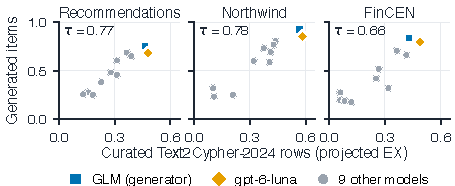
\includegraphics[width=\columnwidth]{figures/curated_agreement.pdf}
\caption{Generated benchmarks order models as curated ones do: each point is one of 11 models, scored zero-shot on 160 generated items ($y$) and on curated rows of the same graph ($x$); permutation $p<0.005$.}
\label{fig:curated}
\end{figure}

\paragraph{Does it rank models like curated benchmarks?} On Recommendations, Northwind, and FinCEN, the ranking of the 11 models on 160 generated items matches their ranking on curated test rows (Figure~\ref{fig:curated}; Kendall $\tau$ 0.77, 0.78, and 0.66), and leaving out the generator changes $\tau$ by at most 0.04. Accuracy is higher on generated items, so we compare only the rankings. GLM and gpt-6-luna swap places on every graph (GLM leads on generated items), but so do two pairs without the generator, so any home advantage is small. The two independently generated halves of the main build also rank the models alike ($\tau=0.89$ [0.82, 1.00]), so regeneration preserves the ranking.

\subsection{Downstream stress test}
\label{sec:downstream}
\begin{table}[t]
\centering
\footnotesize
\setlength{\tabcolsep}{3pt}
\resizebox{\columnwidth}{!}{%
\begin{tabular}{@{}lrrrrrr@{}}
\toprule
& All & \multicolumn{4}{c}{Held-out test (342 items)} & T2C-24 \\
\cmidrule(lr){3-6}
Model & proj. & strict & proj. & gov. & few & proj. \\
\midrule
gpt-6-luna$^\ddagger$ & 0.77 & 0.44 & 0.76 & 0.79 & 0.84 & 0.51 \\
GLM-5.3-Flash$^\dagger$ & 0.77 & 0.48 & 0.80 & 0.74 & 0.86 & 0.49 \\
Gemma-4-26B-A4B & 0.69 & 0.42 & 0.76 & 0.73 & 0.82 & 0.40 \\
gpt-oss-20b & 0.58 & 0.35 & 0.58 & 0.54 & 0.66 & 0.40 \\
Mistral-Small-3.2-24B & 0.51 & 0.36 & 0.52 & 0.47 & 0.70 & 0.32 \\
Qwen3-Coder-30B-A3B & 0.43 & 0.33 & 0.41 & 0.42 & 0.57 & 0.33 \\
Phi-4 & 0.43 & 0.31 & 0.41 & 0.38 & 0.58 & 0.22 \\
Qwen3.5-9B & 0.35 & 0.30 & 0.39 & 0.40 & 0.54 & 0.33 \\
Llama-3.1-8B & 0.24 & 0.23 & 0.27 & 0.22 & 0.40 & 0.12 \\
Gemma-3-12B & 0.21 & 0.11 & 0.16 & 0.13 & 0.51 & 0.18 \\
Gemma-3-4B & 0.21 & 0.17 & 0.22 & 0.17 & 0.34 & 0.11 \\
\midrule
Median (11 models) & 0.43 & 0.33 & 0.41 & 0.42 & 0.58 & 0.33 \\
\midrule
Gemma-3-4B T2C$^\S$ & -- & 0.28 & 0.39 & -- & -- & 0.51 \\
Gemma-2-9B T2C$^\S$ & -- & 0.23 & 0.30 & -- & -- & -- \\
\bottomrule
\end{tabular}}
\caption{Execution accuracy. All: zero-shot projected EX on all 3,038 items (by tier in Appendix Table~\ref{tab:downstream_tiers}). Held-out test: standard prompt (strict and projected EX), governed prompt (gov.), and five same-category train demonstrations that share no signature with the test item (few). T2C-24: 569 curated Text2Cypher-2024 test rows on three public graphs. $^\dagger$generator; $^\ddagger$closed model; $^\S$Neo4j Text2Cypher fine-tunes run locally with their documented prompt (the standard prompt gives 0.27/0.39 and 0.22/0.28). 95\% intervals on all items are about $\pm$0.03 (Appendix Table~\ref{tab:downstream_full}).}
\label{tab:downstream}
\end{table}


On all 3,038 items, zero-shot projected accuracy ranges from 0.21 to 0.77 (Table~\ref{tab:downstream}; median 0.43), far below median parse validity (0.99) and execution success (0.80; Appendix Table~\ref{tab:downstream_full}): models write Cypher that runs but answers a different question, and up to 13\% of predictions traverse a relationship backwards. Tiers calibrated on an earlier benchmark separate the same models on fresh items: every model falls from easy to medium to hard, the median from 0.70 to 0.42 to 0.15 (Appendix Figure~\ref{fig:tiers}). A third of hard references are wrong (\S\ref{sec:validity}), which blurs hard-tier scores, but the gap between the strongest models (0.58--0.61) and the median stays wide.

On the held-out test, five same-category demonstrations help all 11 models (median 0.41 to 0.58) although none shares the test item's signature, while the governed prompt, which adds the generator's own Cypher rules, lowers 8 of 11. Neo4j's Text2Cypher-tuned Gemma-3-4B scores 0.39, up from 0.22 for its base model but below its 0.51 on curated rows from its training distribution: public fine-tuning helps, but much of the gain does not transfer to a new schema.

\subsection{Refresh, small generators, wide schemas}
\label{sec:refresh}
\paragraph{Refresh.} We applied four schema migrations and two data-drift edits to a copy of FinBench and re-executed the 1,882 now \emph{stale} references, those written before the change (Appendix Table~\ref{tab:refresh}). Renaming \cy{TRANSFER\_TO} breaks 562 (30\%) without a single error: 376 return no rows and 165 different rows.
Stale references also flatter models: prompted with the old schema, as by a team that missed the migration, all 11 models score 11 to 23 points higher against stale than against refreshed references (Figure~\ref{fig:refresh}), mostly because outdated predictions and references return the same empty rows. Data drift alone changes 13--16\% of answers. The refresh path rewrites renamed references, re-executes items whose answers changed, and regenerates only items whose structure is gone: after \cy{GUARANTEE} was dropped, it regenerated the 180 affected items for \$0.16, 8\% of the cost and worker time of rebuilding FinBench.

\paragraph{Smaller generators and larger schemas.} With Qwen3.5-9B (one 24\,GB GPU) as generator in a 25-per-cell run, with the larger judges kept, only 30\% of template proposals met the contract and 4 of 16 cells filled; given GLM's questions, though, its references return the released answer on 86\% of items (Appendix~\ref{app:gen9b}). As a test of schema width, we loaded the five public graphs four times each into one database under namespaced labels (132 labels, 148 relationship types): the unchanged pipeline filled all eight 10-item cells at 59\% acceptance and \$2.13 per 1,000 items (Appendix~\ref{app:wide}).


\section{Lessons for Deployment}
\label{sec:lessons}
\textbf{Let the graph decide.} LLMs propose query structures well but do not know what the data contains. Filling slots by reverse querying cut empty-result rejections from 24\% to 1.3\% of candidates and gives every item an observed answer; an empty reference rewards any wrong query that also returns nothing, which is exactly how stale references inflated scores.

\begin{figure}[t]
\centering
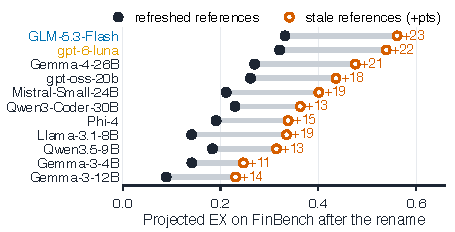
\includegraphics[width=\columnwidth]{figures/refresh_inflation.pdf}
\caption{Stale references inflate scores: after \cy{TRANSFER\_TO} is renamed, models prompted with the old schema score 11 to 23 points higher against stale references (open) than against refreshed ones (filled).}
\label{fig:refresh}
\end{figure}

\textbf{Spend judgment last.} Ordering checks by cost keeps a strict panel affordable: 60\% of rejected candidates never reached a judge.

\textbf{Write the conventions down.} Many disagreements about correctness are disagreements about how to read a question. Giving the judge this sheet and a checklist raised its agreement with adjudicated labels from $\kappa=0.14$ to 0.61--0.67 on our design items; a team adds its own rules there.

\textbf{Measure validity independently.} Every item in our human sample had passed both judges, yet one reference in seven is wrong, and one in three among hard items. An outside auditor that flags a fifth of the release catches about three in four wrong references, so its flags and hard items should go to human review. An open-weight auditor can do this privately: DeepSeek-V4.1-Flash caught 8 of our sample's 12 wrong references (Appendix~\ref{app:sensitivity}).

\textbf{Make refresh part of the benchmark.} Migrations break stale references silently: they return empty rows that outdated predictions match, so scores rise where the benchmark has stopped measuring.

\textbf{Match the model to the step.} Proposing templates is the hard step, and writing a reference for a given question is far easier: a 9B model failed at the first and mostly succeeded at the second.

\section{Conclusion}
PIPE-Cypher turns a live property graph into a private Text-to-Cypher benchmark that an organization can rebuild whenever its graph changes, with open-weight models it can host. Execution-verified bindings, deterministic checks, explicit answer conventions, and a cross-family judge panel yield references that a human audit finds 81\% correct and 14\% wrong, with the errors concentrated in hard items that an outside auditor can route to review. The benchmark ranks models as curated benchmarks do, and it stays useful under change: after a schema migration, stale references inflated every model's score by 11 to 23 points, while regenerating only the affected items cost 8\% of a rebuild. The next step is a proprietary graph, where the analysts who ask the questions can judge the benchmark (Appendix~\ref{app:tenant}).

\section*{Limitations}
All graphs in this study are public; we did not run PIPE-Cypher on a proprietary tenant graph, and Appendix~\ref{app:tenant} explains why we expect the results to carry over and what a tenant should check first. The eight categories are a balancing scaffold; we did not measure how tenant questions are distributed. Neo4j~5 is the backend of every experiment, and we did not run on another engine. Cypher is also available as openCypher on Amazon Neptune, Memgraph, Apache AGE, and SAP HANA Graph, among others, and nothing in the method depends on Neo4j: the pipeline reaches the graph through one client that issues read-only queries, and its Neo4j-specific parts are confined to that client and the schema reader (two introspection procedures and the syntax check), which a schema file can replace. Engines differ in functions and dialect details, so a port should first rerun the deterministic checks on its own engine. Every item is a single question with one reference query; multi-turn sessions, which conversational benchmarks such as CypherTurn~\citep{cypherturn2026} evaluate, are outside our scope. Reverse querying keeps the values whose query returns an answer, which favors well-connected entities; a cap on the share of a category's items that may mention one entity (8\%) limits this, and we did not measure the skew that remains. PIPE-Cypher benchmarks the read-only subset of Cypher and skips rewrites around \cy{CALL}, \cy{UNION}, and \cy{UNWIND}. The judge panel was designed on items labeled by an LLM adjudicator, and the difficulty tiers were fitted to the same 11 models we evaluate. Human validation covers 70 items, so per-slice error rates have wide intervals. Its annotators are two of the authors, because deciding whether a query answers a question requires reading Cypher and knowing the graph's schema; audits of text-to-SQL references rely on SQL experts for the same reason~\citep{wretblad2024noise,jin2026pervasive}. To limit bias, labeling was blind to verdicts and sampling reasons, one annotator did not work on the pipeline, and we report agreement on the shared items before discussion. Annotators who know the system may still be more lenient than outsiders, so the error estimate should be read together with the outside auditor's flags. An estimated 14\% of released references are wrong, mostly on hard items, so part of the hard tier's low accuracy reflects reference errors; keeping only items the auditor passes removes most of them at the cost of a fifth of the items. The two regenerated halves share seed and schema-derived templates and the generator, so their agreement measures sampling variation only. Because a binding must yield a non-degenerate answer, single-number answers are almost never zero (5 of 550), although yes/no answers are balanced (57\% yes). Questions whose right answer is zero or an empty list, which monitoring and compliance work asks often, are therefore under-represented, and a tenant that needs them should add such templates deliberately. Both accuracy metrics measure execution agreement on the current graph: queries with different meanings can return the same rows when the data hold no case that separates them, as four of our seven corrected references did, and projected EX also tolerates differences in column naming and context columns (Appendix~\ref{app:sensitivity}). They compare row sets and do not score row order; scoring it on the 249 items that ask for a sorted listing lowers accuracy by at most 1.25 points and does not change the ranking (Appendix~\ref{app:sensitivity}). Every model that decides what enters the benchmark has open weights, so the pipeline can run entirely on an organization's own hardware; because our graphs are public we reached them through hosted endpoints, and the smallest generator we tested, Qwen3.5-9B, fits one 24\,GB GPU. We also used one closed model, gpt-6-luna, as outside auditor, replay generator, and downstream reference. A model at the frontier of capability and cost is a useful yardstick for the open-weight components, and none of its roles is needed to build or release a benchmark. An on-premises deployment would give the auditor role to an open-weight model, and the strongest one we tested, DeepSeek-V4.1-Flash, catches 8 of the 12 wrong references where gpt-6-luna catches 10 (Appendix~\ref{app:sensitivity}). The redaction audit checks residuals of values the pipeline produces; it does not classify PII or hide schema names.

\section*{Ethics Statement}
PIPE-Cypher is designed for private benchmark generation in which graph data stays within an organization's boundary. All graphs in this study are public or synthetic, which is why hosted model endpoints could be used; deployments on private graphs should host the open-weight models themselves. Organizations should restrict benchmark artifacts to authorized users and review sampled values. The human labels were provided by two of the authors on public or synthetic graph data; no outside annotators were recruited or paid. The labeling page recorded only an account identifier per label, and labels are reported in aggregate.

\section*{Code and Data}
The pipeline code, the generated benchmarks, the predictions of all evaluated models, the result files, and the human-labeled items are available at \url{https://github.com/suraj-ranganath/PIPE-Cypher}, and the benchmarks are also on the Hugging Face Hub at \url{https://huggingface.co/datasets/suraj-ranganath/PIPE-Cypher-benchmarks}. The release marks every item with the outside auditor's verdict, so the 2,264 items it passed can be used as an audited subset.

\bibliography{references}

\clearpage
\appendix
\raggedbottom
% Appendix: deployment path on a tenant graph.

\section{From Public Graphs to a Tenant Graph}\label{app:tenant}
We could not run PIPE-Cypher on a proprietary graph: we had neither a tenant's data nor its hardware. This appendix explains why the results should carry over and what a tenant would check first.

\paragraph{The pipeline only reads three things from a tenant.} These are a read-only connection, the schema found by introspection, and a value policy (which properties may expose sample values, how many, and how long). Nothing in the pipeline is specific to FinBench or SNB:
\begin{itemize}
\item Templates are proposed by the generator from the schema, or derived from the schema itself.
\item Slot values are drawn from the tenant's graph through the template's own query and are kept only if that query returns a non-empty answer.
\item Every deterministic check either inspects the Cypher text (read-only, schema, direction, categorical values, ties at the \cy{LIMIT} cutoff, literal consistency) or executes the query on the tenant's graph.
\end{itemize}
Seed questions and query logs are optional inputs. The convention sheet (\S\ref{sec:prompt_contracts}) is a plain-text file that a tenant can edit.

\paragraph{Evidence that the design carries over.} Table~\ref{tab:tenant_evidence} maps each requirement of a tenant deployment to a measurement in this paper.

\begin{table}[H]
\centering\small
\begin{tabular}{@{}p{0.36\linewidth}p{0.58\linewidth}@{}}
\toprule
Tenant requirement & Evidence \\
\midrule
New schema, no hand-written templates & Three Text2Cypher-2024 graphs onboarded from introspection alone; the generated sets rank 11 models like curated ones (Kendall $\tau$ 0.66--0.78). \\
Answers grounded in tenant data & Every slot value is verified by running its template's query; empty-result rejections fall from 24\% (v2) to 1.3\% of candidates. \\
References that do not depend on one model & Given the same questions, gpt-6-luna's references return the generator's answer on 95\% of items, as often as a second generator run (94\%), and GLM gains at most 2.4 points from being scored against its own references (95\% CI includes zero). \\
Self-hosted models & Qwen3.5-9B, which fits one 24\,GB GPU, writes references that agree with GLM's on 86\% of fixed plans; as template author it needs seed templates (Appendix~\ref{app:gen9b}). \\
Values stay private & Value-sampling policy plus a residual audit: 36 of 12,695 sensitive values (0.28\%) remain in the redacted export, all literals the generator wrote into Cypher outside a slot (mostly place names and a label name). \\
Affordable to run & \$1.15 and about 25 minutes per 1,000 items on hosted endpoints with 32 parallel workers on a laptop, with 37\% of prompt tokens reused from cache. \\
Large schemas & On a 132-label, 148-type merged graph the unchanged pipeline fills every cell at 59\% acceptance and about twice the cost per item (Appendix~\ref{app:wide}). \\
Graphs change & Refresh run end to end on a migrated copy: renamed references are rewritten (557 of 562 keep their answer) and only the 180 items touching a dropped relationship are regenerated, at 8\% of a full FinBench rebuild's cost and worker time. \\
\bottomrule
\end{tabular}
\caption{What a tenant deployment needs and where this paper measures it.}
\label{tab:tenant_evidence}
\end{table}

\paragraph{What will differ on a tenant graph, and the existing control for it.}
\begin{itemize}
\item \emph{Messier schemas} (sparse or free-text properties, inconsistent names): introspection caps categorical values and omits free-text properties. Templates that use properties absent from the schema are rejected and logged.
\item \emph{Sensitive values}: the value policy and the redaction audit above. Exports for sharing are redacted, and raw artifacts stay inside the tenant's boundary.
\item \emph{Domain conventions} (``active customer'', fiscal periods, how to count accounts): conventions are added to the sheet, which both the question writer and the judges read.
\item \emph{A different mix of questions}: the eight categories are a balancing scaffold. Seed templates can come from a query log, so a tenant's own question mix can replace or reweight the planner's targets.
\item \emph{Larger schemas}: the 132-label test shows the cost (a longer schema prompt, about twice the cost per item) and the new failure mode (properties attached to the wrong label, caught by the schema check). Beyond a few hundred labels, each prompt would carry only the labels within a few hops of the template's pattern, and domain quotas would sit next to category quotas.
\end{itemize}

\paragraph{Models and backend on premises.} The generator and both judges have open weights, so a tenant can serve them on its own hardware and no graph content leaves its boundary. In this study the graphs are public, which let us reach those models through hosted endpoints and add a closed frontier model, gpt-6-luna, in three roles that never decide what is released: outside auditor, replay generator, and downstream reference. It serves as a yardstick at the frontier of capability and cost against which the open-weight components can be read. A tenant that cannot use a closed model gives the auditor role to an open-weight one (Table~\ref{tab:openauditor}) and loses the other two roles, which are measurements for this paper. The graph engine is similarly replaceable in principle: the pipeline needs read-only Cypher execution and a schema, both available on openCypher engines such as Amazon Neptune, Memgraph, and Apache AGE, although we ran only Neo4j~5 and a port would start by rerunning the deterministic checks.

\paragraph{Recommended rollout.}
\begin{enumerate}
\item Dry run with 10 items per category.
\item Apply the go/no-go checks used for our pilot: empty-result rate below 5\%, zero ties and literal mismatches, the mix of difficulty tiers, judge agreement, question similarity, the redaction residual, and projected cost.
\item Tenant analysts review 50 items, using our labeling interface.
\item Full build.
\item Scheduled refresh whenever the schema migrates.
\end{enumerate}
The quantity we have not measured is how useful tenant analysts find the benchmark. These are the checks we would run first to measure it.


\section{Running Example, Glossary, Models, and Prior Work}
Table~\ref{tab:glossary} defines the terms we use, Table~\ref{tab:running_example} traces the item of Figure~\ref{fig:pipeline} through every stage, Table~\ref{tab:models} lists the models and how they were served, and Table~\ref{tab:prior_mechanism_comparison} relates PIPE-Cypher to the mechanisms of prior work.
\begin{table}[H]
\centering
\footnotesize
\begin{tabular}{@{}p{2.25cm}p{4.95cm}@{}}
\toprule
Term & Meaning in this paper \\
\midrule
Parameterized template & An LLM-proposed question with typed slots plus Cypher that uses each slot as a \cy{\$slot} parameter. \\
Verified binding & A slot value drawn through the template's own query and kept only if that query, run with it, returns a non-degenerate answer. \\
Query signature & A Cypher query with literals and variable names abstracted; two items with the same signature differ only in values. \\
Signature / tier quota & Maximum accepted items per signature, and per difficulty tier, in a graph--category cell. \\
Difficulty tier & Easy, medium, or hard from a structural score calibrated on how often models solved earlier items. \\
Template induction & Asking the LLM for templates with uncovered structure, or at a short tier, once existing templates saturate. \\
Convention sheet & Thirteen plain-text reading rules shared by question writer, generator, judges, auditor, and annotators. \\
Deterministic checks & Code checks before the judge (symmetric relationship types such as SNB's \cy{KNOWS} are matched without a direction): read-only, schema, direction, categorical and literal consistency, \cy{LIMIT} ties, category contract, structural defects, emptiness, quotas. \\
Judge panel & Two cross-family LLM judges answering a nine-item checklist; both must accept. \\
Outside auditor & A judge (gpt-6-luna) that does not decide what is released; used to estimate errors in released items. \\
Pipeline-validated reference & An exported query that passed every check; its correctness is measured separately. \\
Strict / projected EX & Exact row-set match / match on the answer columns, ignoring column names, order, extra columns, and policy context columns. \\
Template-held-out split & Test items whose signatures never occur in train. \\
\bottomrule
\end{tabular}
\caption{Terms used throughout the paper.}
\label{tab:glossary}
\end{table}

% Appendix: the running example from Figure 1, stage by stage.
\begin{table*}[!t]
\centering
\footnotesize
\begin{tabular}{@{}>{\raggedright\arraybackslash}p{2.1cm}>{\raggedright\arraybackslash}p{13.4cm}@{}}
\toprule
Stage & Running example (FinBench, category \emph{path/temporal}, tier \emph{hard}) \\
\midrule
1 Profile & Introspection records \cy{(:Account)-[:TRANSFER\_TO \{createTime, amount\}]->(:Account)}, typed properties, and bounded categorical values. \\
2 Plan & Target: 250 path/temporal FinBench items in two halves; tier quota 5/25/70\% easy/medium/hard; at most 8 items per query signature in each half. \\
3 Propose & The LLM proposes \emph{``How many transfers did account \{account\} make to a different account between 2020-01-01 and 2020-12-31?''} with\newline \cy{MATCH (a:Account \{accountId: \$account\})-[r:TRANSFER\_TO]->(b:Account) WHERE a <> b AND r.createTime >= datetime('2020-01-01')}\newline \cy{AND r.createTime <= datetime('2020-12-31') RETURN DISTINCT count(r) AS numTransfers} \\
4 Bind \& verify & Candidates come from the template query rewritten to return \cy{a.accountId}; \cy{account = 4709076360369276476} is kept because the query then returns 2 (a count of 0 is rejected). Structural score 18: hard tier. \\
5 Realize & Register \emph{imperative}: \emph{``List the number of transfers made by account with id 4709076360369276476 to a different account between 2020-01-01 and 2020-12-31.''} The generator's reference ends the window at \cy{2020-12-31T23:59:59}, so the whole last day counts (C7); here it returns the same answer as the template query. \\
6 Checks & Read-only, schema, direction checks; every stated value (id, both dates) appears in the Cypher and no other literal does; ``different account'' is \cy{a <> b} (convention C10). \\
7--8 Execute, judges & Non-degenerate answer; no tie at a cutoff; hard-tier and signature quotas not full; neither judge answers any checklist item ``no''. \\
Evaluate & Prediction and reference are both executed; a prediction returning the count 2 under any column name scores 1 (single-column answers are compared by value). \\
\bottomrule
\end{tabular}
\caption{The running example of Figure~\ref{fig:pipeline}, traced through all eight stages. Identifiers are from the LDBC synthetic data generator.}
\label{tab:running_example}
\end{table*}

\begin{table*}[!t]
\centering
\footnotesize
\setlength{\tabcolsep}{4pt}
\begin{tabular}{@{}>{\raggedright\arraybackslash}p{4.3cm}>{\raggedright\arraybackslash}p{1.9cm}>{\raggedright\arraybackslash}p{3.85cm}>{\raggedright\arraybackslash}p{3.1cm}>{\raggedright\arraybackslash}p{1.7cm}@{}}
\toprule
Model (weights) & Family & Role & Precision served & Prompt formats \\
\midrule
GLM-5.3-Flash (zai-org/GLM-5.3-Flash, MIT) & GLM & generator, judge 1; downstream$^\dagger$ & FP8 (released), one pinned provider & standard, governed \\
Qwen3.5-9B & Qwen & 9B generator ablation; replay generator; downstream & BF16 & standard, governed \\
Llama-3.1-8B-Instruct & Llama & downstream & BF16 & standard, governed \\
Gemma-3-4B-IT, Gemma-3-12B-IT & Gemma & downstream & BF16 & standard, governed \\
Gemma-4-26B-A4B-IT & Gemma & judge 2; downstream & BF16, one pinned provider & standard, governed \\
Phi-4 & Phi & downstream & BF16 & standard, governed \\
Mistral-Small-3.2-24B-Instruct & Mistral & downstream & BF16 & standard, governed \\
gpt-oss-20b & gpt-oss & downstream (open-weight reasoning) & BF16 as served (released in MXFP4) & standard, governed \\
Qwen3-Coder-30B-A3B-Instruct & Qwen & downstream & FP8 (official release) & standard, governed \\
Neo4j text-to-cypher Gemma-3-4B (2025.04) & Text2Cypher-tuned & downstream & BF16 (local, MLX) & standard, native \\
Neo4j text2cypher Gemma-2-9B LoRA (2024v1) & Text2Cypher-tuned & downstream & BF16, LoRA merged (local, MLX) & standard, native \\
gpt-6-luna (hosted, closed) & OpenAI GPT & outside auditor; replay generator; downstream reference & provider default & standard, governed \\
\bottomrule
\end{tabular}
\caption{Models. All open-weight models are deployable inside an organization's boundary; in this study, models without local hardware were reached through hosted endpoints serving their released precision or higher (no FP4/INT4 re-quantization), and only on public graphs. $^\dagger$Generator family. ``Governed'' adds the answer conventions the generator saw (context columns, direction, exact literals); ``native'' is the checkpoint's documented model-card or official-notebook prompt.}
\label{tab:models}
\end{table*}

\clearpage
\begin{table}[H]
\centering
\footnotesize
\begin{tabular}{@{}p{0.37\columnwidth}p{0.56\columnwidth}@{}}
\toprule
Prior mechanism & PIPE-Cypher delta \\
\midrule
Template/LLM synthesis in SyntheT2C~\citep{synthet2c2025} and Auto-Cypher~\citep{autocypher2025} & Outcome-aware reverse grounding binds slots through live Cypher before NL realization. \\
Execution validation in Auto-Cypher~\citep{autocypher2025} and Mind the Query~\citep{mindthequery2025} & Execution is one check in a ledger with direction, read-only, value, non-empty, and judge evidence. \\
Schema/value checks in Mind the Query~\citep{mindthequery2025} & Checks are packaged for private refresh with configurable value sampling and redacted exports. \\
Human logical review in Mind the Query~\citep{mindthequery2025} & Validity is tested independently (generator swap, cross-family judges, ranking agreement with curated sets); human labels are an optional audit after generation. \\
Public static datasets and tuning corpora~\citep{text2cypher2025,cypherbench2025,text2cypher2024dataset} & Organization-run benchmark factory with manifests, refresh, and provenance audits. \\
\bottomrule
\end{tabular}
\caption{Prior mechanism comparison. PIPE-Cypher combines outcome-aware grounding, deterministic Cypher checks, independent validity tests, privacy policy, refresh support, and audit logs so organizations can generate benchmarks from their own graphs.}
\label{tab:prior_mechanism_comparison}
\end{table}


\section{Generation, Judges, and Privacy}
\label{app:judges}
This appendix compares the three versions of the benchmark (Table~\ref{tab:construction}), isolates the effect of reverse querying (Table~\ref{tab:ablation_binding}), accounts for every candidate, call, and dollar of the main build (Table~\ref{tab:generation}), reports how the judges were chosen and how they behaved (Table~\ref{tab:judges}), and audits the redacted export (Table~\ref{tab:redaction}). Of the 32 cells of the main build (2 graphs $\times$ 8 categories $\times$ 2 halves), 21 reached their target, 3 ran out of templates with bindable slots, and 8 were stopped at a fixed time budget while only full tier quotas were still rejecting candidates; the release reaches 95\% of the planned item count; overall the build accepted 54\% of its candidates, and the two judges account for \$1.86 of its \$3.50.
\begin{table}[H]
\centering
\footnotesize
\setlength{\tabcolsep}{3pt}
\resizebox{\columnwidth}{!}{%
\begin{tabular}{@{}lrrr@{}}
\toprule
& v1 & v2 & v3 \\
\midrule
Items (FinBench / SNB per category) & 3,000 (250/125) & 2,080 (150/110) & 3,038 ($\leq$250/150) \\
Candidates $\rightarrow$ accepted & -- & 5,031 $\rightarrow$ 2,609 & 5,617 $\rightarrow$ 3,042 \\
Empty-result rejections (\% of candidates) & -- & 24.2\% & 1.3\% \\
Released refs.\ with a \cy{LIMIT}-cutoff tie & -- & 65 & 0 \\
Released items with a literal mismatch & -- & 201 (9.7\%) & 0 \\
Query signatures & 123 & 1,312 & 919 \\
Signatures per cell (min / median) & 1 / 1 & 19 / 75 & 19 / 54 \\
Top-10 signature share & 67.3\% & 3.8\% & 4.3\% \\
Distinct-2 / EAD-Distinct-2 & 0.09 / 0.27 & 0.24 / 0.70 & 0.19 / 0.73 \\
Self-BLEU-2, sampled (lower is better) & 0.81 & 0.87 & 0.78 \\
Easy / medium / hard, calibrated (\%) & 30 / 59 / 11 & 33 / 41 / 26 & 35 / 36 / 29 \\
Test items sharing a train signature & 289 / 296 & 0 / 216 & 0 / 342 \\
API cost per 1,000 items & local & \$1.55 & \$1.15 \\
\bottomrule
\end{tabular}}
\caption{Three generations of the FinBench/SNB benchmark: v1, the first version, drew its 3,000 items from a small fixed template set; v2 is the baseline of \S\ref{sec:setup}. v3 binds slots through each template's own query, checks literals and \cy{LIMIT} ties before the judge, and rewrites questions in four registers: empty-result rejections fall from 24\% to 1.3\% of candidates and no released item has a tie or literal mismatch. Tiers use the calibrated score for all three versions (v2's heuristic had reported 1\% hard). v3 reuses each verified template for several bindings (3.3 items per signature vs.\ 1.6), so it has fewer signatures than v2 at the same per-cell floor and a similar top-10 share. Test counts refer to the template-held-out split.}
\label{tab:construction}
\end{table}

\begin{table}[H]
\centering
\footnotesize
\setlength{\tabcolsep}{4pt}
\resizebox{\columnwidth}{!}{%
\begin{tabular}{@{}lrr@{}}
\toprule
& Verified bindings on & Verified bindings off \\
\midrule
Candidates $\rightarrow$ accepted & 1,030 $\rightarrow$ 392 (38\%) & 1,104 $\rightarrow$ 395 (36\%) \\
Rejected for an empty result & 16 (1.6\%) & 397 (36.0\%) \\
Rejected: tier quota full & 313 & 179 \\
Rejected: entity-diversity cap & 171 & 36 \\
Rejected: tie at a \cy{LIMIT} cutoff & 36 & 51 \\
Rejected: slot bindings unavailable & 31 & 2 \\
Rejected: literal mismatch & 23 & 22 \\
Rejected by the judge panel & 14 & 8 \\
Cells reaching 25 items (of 16) & 13 & 14 \\
API cost & \$0.65 & \$0.68 \\
\bottomrule
\end{tabular}}
\caption{One-component ablation of reverse querying: the current pipeline at 25 items per category on FinBench and SNB (16 cells, seed 1), with slot values verified through the template's own query (on) or drawn from the earlier property lookup without verification (off); everything else is identical. Without verification, more than a third of all candidates return nothing. At this small target both arms accept a similar share overall, because with verification on the rejections move to the quotas: verified templates yield several valid bindings each, which then meet the tier quota and the cap on how often one entity may appear.}
\label{tab:ablation_binding}
\end{table}

\begin{table*}[t]
\centering
\small
\setlength{\tabcolsep}{4pt}
\begin{tabular}{@{}lrr@{}}
\toprule
& v2 & v3 \\
\midrule
Candidates / accepted & 5,031 / 2,609 & 5,617 / 3,042 \\
Exported & 2,080 & 3,038 \\
\multicolumn{3}{@{}l}{\emph{First blocking reason for rejected candidates}} \\
Tier quota full & -- & 1,713 \\
LLM judge / panel reject & 405 & 197 \\
Slot bindings unavailable & 385 & 181 \\
Duplicate, entity, or signature cap & 385 & 138 \\
Tie at the \cy{ORDER BY\ldots LIMIT} cutoff & -- & 131 \\
Category contract (e.g., yes/no returns one boolean) & -- & 98 \\
Empty result & 1,220 & 72 \\
Literal mismatch (question vs.\ Cypher) & -- & 22 \\
Structural defect (unlisted pattern, dropped variable) & -- & 22 \\
Execution, schema, or syntax error; unordered \cy{LIMIT} & 27 & 1 \\
\multicolumn{3}{@{}l}{\emph{Templates}} \\
LLM proposals kept / proposed & -- & 826 / 1,081 \\
Accepted items: seed / schema-derived / LLM / induced & 279 / 896 / 1,247 / 187 & 375 / 423 / 1,476 / 768 \\
\multicolumn{3}{@{}l}{\emph{Cost and time}} \\
LLM calls (generation / judge 1 / judge 2) & 18,405 & 11,086 / 4,368 / 4,362 \\
Prompt / completion / reasoning tokens & 20.7M / 1.39M / 0.70M & 57.0M / 5.11M / 0.54M \\
Prompt tokens served from cache & 22\% & 37\% \\
API cost (generation / judge 1 / judge 2) & \$3.23 & \$1.63 / \$1.42 / \$0.44 \\
Cost per 1,000 exported items & \$1.55 & \$1.15 \\
Wall-clock (parallel workers, one laptop or CPU host) & 54 min & 76 min \\
\bottomrule
\end{tabular}
\caption{Generation accounting for the FinBench/SNB builds. In v3 the deterministic checks run before the judges: 1,142 of the 1,713 tier-quota rejections, and 60\% of all rejections, cost no judge call, while 475 candidates passed the panel and were then rejected when the tier quota was re-checked at acceptance. Judge calls therefore exceed the 3,239 candidates whose final verdict came from the panel; candidates whose generator reference was rejected were also judged again with their template's Cypher. Empty results, v2's dominant failure (LLM-proposed templates whose slots fell back to a generic value lookup), drop from 1,220 to 72. v3 sends about three times as many prompt tokens (full schema and convention sheet in every judge prompt, two judges) yet costs less per item, because its GLM endpoint is cheaper and caches prompt prefixes.}
\label{tab:generation}
\end{table*}

\begin{table*}[t]
\centering
\small
\setlength{\tabcolsep}{3pt}
\begin{tabular}{@{}lrrr@{}}
\toprule
\multicolumn{4}{@{}l}{\emph{(a) Choosing the judge: 150 disagreement-oversampled v2 items, adjudicated labels}} \\
Judge and prompt & Agreement [95\% CI] & $\kappa$ & False acc.\,/\,rej. \\
\midrule
GLM, v2 free-form prompt & 0.55 [0.47, 0.63] & 0.14 & 55 / 12 \\
GLM, v3 checklist + convention sheet & 0.83 [0.77, 0.88] & 0.67 & 22 / 3 \\
Gemma-4-26B-A4B, v3 checklist & 0.73 & 0.48 & 38 / 2 \\
gpt-oss-20b, v3 checklist & 0.74 & 0.48 & 22 / 17 \\
\textbf{Panel GLM + Gemma-4 (both must accept)} & \textbf{0.87 [0.80, 0.91]} & \textbf{0.73} & 15 / 5 \\
Panel GLM + gpt-oss-20b & 0.80 & 0.59 & 10 / 20 \\
\midrule
\multicolumn{4}{@{}l}{\emph{(b) The panel on the v3 build (3,239 judged candidates)}} \\
\multicolumn{3}{@{}l}{Pass rate: GLM / Gemma-4 / both} & 95.6 / 96.6 / 93.9\% \\
\multicolumn{3}{@{}l}{Agreement between the two judges ($\kappa$; prevalence-adjusted $\kappa$)} & 95.6\% (0.41; 0.91) \\
\midrule
\multicolumn{4}{@{}l}{\emph{(c) Outside auditor: gpt-6-luna, same checklist and evidence, audit only}} \\
\multicolumn{3}{@{}l}{Accepted items flagged (easy, medium, hard)} & 21.8\% (11.5, 20.1, 36.5\%) \\
\multicolumn{3}{@{}l}{Agreement with the panel decision ($\kappa$)} & 79.0\% (0.27) \\
\multicolumn{3}{@{}l}{On the 150 adjudicated items: agreement ($\kappa$); false acc./rej.} & 0.86 (0.71); 3 / 18 \\
\bottomrule
\end{tabular}
\caption{Judges. (a) Labels came from an LLM adjudicator that read each item against the convention sheet; the set over-represents v2 defects and judge disagreements, and it also guided four prompt revisions, so these are in-sample design numbers (a frozen rerun of the GLM checklist gave $\kappa=0.61$). The GLM\,+\,Gemma panel was frozen before the build. (b) Both judges pass most v3 candidates, so $\kappa$ understates their agreement. (c) gpt-6-luna is strict: it rejects 26\% of the items adjudicated correct (and accepts 3 of 81 bad ones), so its flag rate overstates the error rate. Most frequent failing criteria: no extra constraints (258), relationships (225), aggregation (193), unambiguous (139). Human labels (\S\ref{sec:validity}) measure how many flags are real.}
\label{tab:judges}
\end{table*}

\begin{table}[H]
\centering
\footnotesize
\resizebox{\columnwidth}{!}{%
\begin{tabular}{@{}lrr@{}}
\toprule
Release (numeric-literal redaction on) & v2 & v3 \\
\midrule
Items & 2,080 & 3,038 \\
Sensitive values audited & 7,740 & 12,695 \\
Residual values after redaction & 81 (1.0\%) & 36 (0.28\%) \\
Items with any residual & 26 & 18 \\
\bottomrule
\end{tabular}}
\caption{Exact-match redaction audit (entity bindings, quoted and numeric Cypher literals, binding-query literals, result-row strings). The 36 v3 residuals are literals the generator wrote directly into the Cypher, outside any slot: continent and country names (Asia, India; 18), the label name Person used as a value (14), and one university name and one forum title (4). With strings-only redaction, v2 had left 11.9\% of values because many slots are numeric identifiers; v3 configurations enable numeric-literal redaction by default.}
\label{tab:redaction}
\end{table}


\section{Calibrated Difficulty}
\label{app:difficulty}
The tier of an item comes from a structural score on its reference Cypher (string literals masked): $\mathrm{score}=\sum_f w_f \min(x_f, c_f)$, with easy $<10\le$ medium $<17\le$ hard. Weights were fitted by non-negative ridge regression of hardness (one minus the share of 11 models that solve an item zero-shot) on the 216 v2 held-out test items, with $\lambda$ chosen by five-fold cross-validation grouped by query signature, then rescaled so that one returned column is worth 2 points and rounded (Table~\ref{tab:difficulty_weights}). WITH stages, OPTIONAL MATCH, and the number of aggregates received zero weight.

\begin{table}[H]
\centering
\footnotesize
\resizebox{\columnwidth}{!}{%
\begin{tabular}{@{}lrr@{}}
\toprule
Feature & Weight & Cap \\
\midrule
Returned columns & 2 & 6 \\
Relationship hops & 2 & 4 \\
Variable-length paths & 2 & 2 \\
Negation (\cy{NOT}, \cy{<>}) & 2 & 2 \\
Relationship-property or path-function reads & 2 & 3 \\
Grouping keys next to an aggregate & 1 & 3 \\
Temporal properties or functions & 1 & 3 \\
\cy{ORDER BY} & 1 & -- \\
\cy{UNWIND} / \cy{collect} & 1 & 2 \\
\cy{WHERE} conjuncts and inline property filters & 1 & 4 \\
Distinct node labels & 1 & 4 \\
\midrule
\multicolumn{3}{@{}p{1.05\columnwidth}@{}}{Out-of-fold Spearman with hardness: 0.56 (old heuristic 0.28; query length alone 0.58)} \\
\multicolumn{3}{@{}p{1.05\columnwidth}@{}}{Out-of-fold solve rate, easy / medium / hard: 0.65 / 0.31 / 0.18} \\
\bottomrule
\end{tabular}}
\caption{Difficulty score. On the calibration items the solve rate falls from easy to medium to hard for all 11 models; of the 43 items no model solved, 24 are hard and 2 easy. The previous heuristic labeled 1 of 216 items hard.}
\label{tab:difficulty_weights}
\end{table}

\paragraph{Quotas.} Tiers track category but are not identical to it, so the planner sets a tier mix per category (e.g., simple retrieval 65/30/5\%, ranking 15/50/35\%, path/temporal 5/25/70\%) chosen so that the whole benchmark targets 35/35/30. Candidates in a full tier are rejected before the judge, and the quota is checked again at acceptance; after 75\% of a cell's attempt budget, unmet quota may move to an adjacent tier, and every such move is recorded. The v3 release reached 35/36/29\%; two of the 24 cells that ran to completion moved quota between tiers (at most six items per tier). We did not use query length, which correlates about as well, because it rewards verbose aliasing. The tiers were fitted to the same 11 models that we later evaluate; the transfer evidence is that their order holds on fresh v3 items (\S\ref{sec:downstream}).


\section{Human Validation Protocol}
\label{app:human}
\paragraph{Sample.} 70 items were drawn from the v3 release, stratified by graph~$\times$ category~$\times$ tier. Within each of these cells, items that none of the 11 models solved zero-shot or that the outside auditor rejected formed a separate stratum with twice the inclusion weight, and hard cells had twice the weight. A sample of 70 cannot cover all 92 resulting strata, so within a cell the smallest stratum was merged into its sibling (smallest first) until 66 strata remained; every cell and every released item is then covered, and inclusion probabilities stay exact. Each of two annotators received 50 items; 30 items were shared to measure agreement between them. The sample holds 41 FinBench and 29 SNB items (21 easy, 22 medium, 27 hard); 23 were rejected by the auditor and 5 were solved by no model.

\paragraph{Annotators.} Both annotators are authors. Judging a reference requires reading Cypher fluently and knowing the FinBench and SNB schemas, including relationship directions and which types are symmetric, so we chose annotators with that background over crowd workers. One annotator did not work on the generation pipeline. They labeled independently without discussing items, did not open the sampling key or any model or judge outputs before finishing, and did not change their individual labels after estimates were computed.

\paragraph{What annotators saw.} A private web page showed one item at a time: the question, the reference Cypher, the first five result rows, the schema elements the query touches (with symmetric relationship types marked), and the convention sheet. A collapsed panel held, for reference, the full prompt the two judges received for that item (their instructions and nine-criterion checklist, the whole graph schema, and the item with its parser features and validator notes), rendered by the judge's own prompt function. Annotators did not answer the checklist. The page did not show the category, calibrated tier, model predictions, any judge verdict, or why the item was sampled.

\paragraph{Labels.} \emph{Question:} clear, or ambiguous (with the convention it leaves open, or ``not covered''). \emph{Reference:} correct; minor issue (the answer is right, but something small is off, such as an extra non-identifying column, a redundant clause, or wording that slightly mismatches the query while the intended answer is clear); or wrong (the query would return a different answer from the one the question asks for: reversed direction, wrong filter or literal, wrong count unit, wrong hop bound, missing or extra rows). A note explained each non-correct label.

\paragraph{Resolving disagreements.} The two annotators' labels differed on 8 of the 30 shared items (6 on the reference, 2 only on the question). After both had finished and the first estimates were computed, they discussed these items together and recorded one label for each; their individual labels were kept, and agreement is reported on them. For each item, a page showed both labels and notes, the conventions at issue, and a corrected query run on the graph beside the reference, with any rows that differed. Two references were resolved as wrong although the corrected query returned the same requested rows on the current graph, because the query answers a different question and would diverge on other data (a single \cy{MATCH} forbids two patterns to share an edge; three companies are not required to differ). One reference that both had labeled wrong was resolved as correct, for a question that admits both readings. Estimates use the resolved labels; Table~\ref{tab:human}a also gives them with the two labels on each shared item averaged instead (an item then counts 0, 0.5, or 1).

\paragraph{Estimates.} Rates are ratio estimates over the 66 strata: each item is weighted by its inverse inclusion probability, and the 95\% interval resamples items with their weights (2,000 resamples). Agreement intervals resample the 30 shared items. Since every released item passed the panel (both panel judges passed all 70 sampled items), one minus the error rate is the panel's precision.

\paragraph{Wrong references.} Of the 12 references resolved as wrong, six omit a constraint or join the question implies or count the wrong unit (three companies are not required to differ; the repayer is not required to be the guaranteed person; a withdrawal to the same account is not excluded; forums are grouped by title and moderator name, which can merge distinct forums; an account linked both ways is counted twice; one \cy{MATCH} forbids two patterns to share an edge). Three answer a question the schema cannot express as asked (summing investment ratios as amounts, requiring an account to receive a repayment, locating a transfer within a sign-in). One encodes a date cutoff wrongly, and two take a reading the convention sheet rules out or leaves open (averaging over accounts with no transfers; what counts as the owner's own account). The auditor flagged 10 of the 12; the two it passed are the ones on which the annotators had first disagreed. Of the 5 items no model solved, 2 have wrong references. Of the auditor's 23 flags, 15 mark some defect (Table~\ref{tab:human}d).

\begin{table}[H]
\centering\small
\setlength{\tabcolsep}{3pt}
\begin{tabular}{@{}lcc@{}}
\toprule
\multicolumn{3}{@{}l}{\emph{(a) Release estimates, \% (95\% CI)}} \\
 & Resolved & Averaged \\
\midrule
Reference wrong & 13.8 [6.3, 22.2] & 15.7 [7.2, 25.6] \\
Wrong or minor issue & 18.8 [10.2, 29.1] & 20.9 [10.8, 32.7] \\
Question ambiguous & 11.8 [4.3, 21.8] & 10.8 [4.9, 18.1] \\
Not correct and clear & 24.0 [13.2, 36.1] & 22.6 [12.7, 34.5] \\
\bottomrule
\end{tabular}

\vspace{6pt}
\begin{tabular}{@{}lrrrr@{}}
\toprule
\multicolumn{5}{@{}l}{\emph{(b) By slice, resolved labels, reweighted \%}} \\
 & $n$ & Wrong & Wr./minor & Ambig. \\
\midrule
FinBench & 41 & 18.0 & 26.0 & 19.1 \\
SNB & 29 & 6.9 & 6.9 & 0.0 \\
\addlinespace
Easy & 21 & 2.5 & 14.6 & 13.1 \\
Medium & 22 & 10.0 & 10.0 & 3.8 \\
Hard & 27 & 32.3 & 35.1 & 20.4 \\
\addlinespace
Simple retrieval & 8 & 0.0 & 3.0 & 0.0 \\
Complex retrieval & 10 & 24.8 & 24.8 & 17.5 \\
Simple aggregation & 8 & 5.7 & 25.1 & 5.7 \\
Complex aggregation & 8 & 30.8 & 35.5 & 44.0 \\
Boolean existence & 9 & 7.0 & 10.7 & 3.6 \\
Negation/difference & 7 & 0.0 & 10.1 & 0.0 \\
Path/temporal & 11 & 31.1 & 31.1 & 21.1 \\
Ranking/top-$k$ & 9 & 8.5 & 8.5 & 0.0 \\
\bottomrule
\end{tabular}

\vspace{6pt}
\begin{tabular}{@{}lcc@{}}
\toprule
\multicolumn{3}{@{}l}{\emph{(c) Agreement on 30 shared items, before discussion}} \\
 & Agree & $\kappa$ [95\% CI] \\
\midrule
Reference, three-way & 80\% & 0.51 [0.23, 0.77] \\
Correct vs.\ not & 90\% & 0.73 [0.38, 1.00] \\
Wrong vs.\ not & 83\% & 0.47 [0.00, 0.81] \\
Question clear vs.\ ambiguous & 87\% & 0.00 (AC1 0.85) \\
\bottomrule
\end{tabular}

\vspace{6pt}
\resizebox{\columnwidth}{!}{%
\begin{tabular}{@{}lcc@{}}
\toprule
\multicolumn{3}{@{}l}{\emph{(d) Auditor (gpt-6-luna) vs.\ resolved labels, items}} \\
 & Flagged & Passed \\
\midrule
Reference wrong & 10 & 2 \\
Minor issue & 4 & 2 \\
Correct, question ambiguous & 1 & 2 \\
Correct and clear & 8 & 41 \\
\addlinespace
\% wrong, reweighted & 59.7 [36.0, 77.7] & 3.9 [0.0, 11.0] \\
\bottomrule
\end{tabular}}
\caption{Human validation on 70 sampled items (30 labeled by both annotators). (a)~Error rates reweighted to the 3,038-item release, using resolved labels or averaging the two labels on shared items. (b)~Slices have 7--41 items, so their intervals are wide. (c)~$\kappa$ for the question is 0 because one annotator labeled every shared question clear; AC1 is Gwet's coefficient. (d)~Rows are exclusive; the auditor flags 22\% of the release.}
\label{tab:human}
\end{table}


\section{Reference Quality, Scoring, and Answer Coverage}
\label{app:sensitivity}
\paragraph{Do scores and rankings depend on doubtful references?} We rescored the 11 models, from their existing zero-shot predictions, on subsets of the release with fewer doubtful references (Table~\ref{tab:sensitivity}). Removing the items the outside auditor flags raises every model's accuracy by 2 to 4 points and the hard-tier median from 0.15 to 0.19, and it leaves the ranking nearly unchanged (Kendall $\tau=0.93$ with the full release). The one change among the stronger models is that gpt-6-luna and GLM, 0.01 apart, swap places; since gpt-6-luna is itself the auditor, this subset mildly favors it. On the 58 human-labeled items whose reference was resolved as not wrong the same four models lead in the same order ($\tau=0.84$), although with 58 items a model's accuracy has a 95\% interval of roughly $\pm 0.12$. The auditor-passed subset keeps 79\% of the audited items: 90\% of easy, 80\% of medium, and 65\% of hard ones (FinBench 80\%, SNB 77\%).

\begin{table}[H]
\centering
\footnotesize
\setlength{\tabcolsep}{3.5pt}
\resizebox{\columnwidth}{!}{%
\begin{tabular}{@{}lrrrrr@{}}
\toprule
& Full & Auditor & Auditor & Human: & Human: \\
& release & passed & flagged & not wrong & fully correct \\
\midrule
Items & 3,038 & 2,264 & 614 & 58 & 52 \\
Kendall $\tau$ vs.\ full release & 1.00 & 0.93 & 0.99 & 0.84 & 0.87 \\
Median projected EX & 0.43 & 0.47 & 0.26 & 0.38 & 0.40 \\
\addlinespace
gpt-6-luna & 0.77 & 0.81 & 0.61 & 0.78 & 0.79 \\
GLM-5.3-Flash & 0.77 & 0.80 & 0.62 & 0.76 & 0.77 \\
Gemma-4-26B-A4B & 0.69 & 0.72 & 0.55 & 0.69 & 0.69 \\
gpt-oss-20b & 0.58 & 0.61 & 0.44 & 0.62 & 0.62 \\
Mistral-Small-3.2-24B & 0.51 & 0.54 & 0.34 & 0.47 & 0.48 \\
Qwen3-Coder-30B-A3B & 0.43 & 0.47 & 0.26 & 0.34 & 0.33 \\
Phi-4 & 0.43 & 0.47 & 0.26 & 0.38 & 0.40 \\
Qwen3.5-9B & 0.35 & 0.38 & 0.21 & 0.33 & 0.33 \\
Llama-3.1-8B & 0.24 & 0.27 & 0.10 & 0.19 & 0.21 \\
Gemma-3-12B & 0.21 & 0.24 & 0.06 & 0.21 & 0.21 \\
Gemma-3-4B & 0.21 & 0.23 & 0.09 & 0.21 & 0.19 \\
\addlinespace
Hard-tier median (items) & 0.15 (869) & 0.19 (544) & 0.11 (298) & 0.26 (19) & 0.29 (17) \\
\bottomrule
\end{tabular}}
\caption{Zero-shot projected EX of the 11 models on subsets with fewer doubtful references. The auditor judged 2,878 of the 3,038 released items (the rest had their question text normalized after the audit). Human columns are unweighted and cover the 70 labeled items; the sample oversampled hard and flagged items, so its accuracies are lower than the release's.}
\label{tab:sensitivity}
\end{table}

\paragraph{What changes when wrong references are corrected?} Filtering removes items and so changes what is measured. As a direct test, for the seven sampled references judged wrong on a clear question we wrote a corrected query that applies the fix named in the annotators' notes and nothing else, and rescored the 11 models' stored zero-shot predictions against it (Table~\ref{tab:corrected}). The other five wrong references belong to questions judged ambiguous, three of which ask for facts the schema does not record; they have no single correct reference, so we left them uncorrected, and such items should be dropped or rewritten. Four of the seven corrections return the same rows as the released reference: the query is logically wrong, but the current data contain no case that exposes it. For the other three the answer changes. Across the 77 model--item pairs, no prediction scored wrong becomes right, and four scored right become wrong (two from gpt-6-luna, one each from GLM and Gemma-4), because those predictions repeated the reference's mistake. In this sample, wrong references therefore rewarded a few incorrect predictions and penalized no correct one. gpt-6-luna falls from 5 to 3 of the seven items and still leads, GLM from 1 to 0, and Gemma-4 from 2 to 1; the other eight models are unchanged. Seven items cannot support a rate, and three of them were first labeled differently by the two annotators, so we read this as the direction of the effect: reference errors here slightly flatter the strongest models and leave the ordering of the rest alone.

\begin{table}[H]
\centering
\footnotesize
\setlength{\tabcolsep}{2.5pt}
\resizebox{\columnwidth}{!}{%
\begin{tabular}{@{}>{\raggedright\arraybackslash}p{0.3\columnwidth}>{\raggedright\arraybackslash}p{0.5\columnwidth}ccc@{}}
\toprule
 & & Rows & \multicolumn{2}{c}{Models right} \\
Item & Fix applied & differ & before & after \\
\midrule
Path/temporal, hard & Match two \cy{KNOWS} conditions separately so that they may use the same edge & no & 0 & 0 \\
Ranking/top-$k$, hard & Count each linked account once, in either direction & yes & 0 & 0 \\
Boolean existence, easy & Encode the date cutoff in the stored unit (epoch milliseconds) & no & 7 & 7 \\
Path/temporal, medium & Require the three companies to be distinct & no & 1 & 1 \\
Complex aggregation, hard & Group by the forum itself & yes & 2 & 0 \\
Complex retrieval, hard & Count only repayments from the guaranteed person's own accounts & no & 1 & 1 \\
Complex aggregation, medium & Average only over accounts with an outgoing transfer (C12) & yes & 2 & 0 \\
\bottomrule
\end{tabular}}
\caption{The seven sampled references judged wrong on a clear question, the fix applied to each, whether the corrected query returns different rows on the current graph, and how many of the 11 models are scored right against the released and the corrected reference (zero-shot, projected EX).}
\label{tab:corrected}
\end{table}

\paragraph{Can an open-weight model do the audit?} A private deployment cannot send its items to a closed auditor, so we ran two open-weight models that took no part in construction as auditors on the 70 human-labeled items, with the same checklist prompt and evidence (Table~\ref{tab:openauditor}). DeepSeek-V4.1-Flash flags 17 items and catches 8 of the 12 wrong references; 14 of its 17 flags mark some defect, a higher share than for gpt-6-luna (15 of 23), and 6\% of the items it passes are wrong (gpt-6-luna: 4\%). Qwen3-Coder-30B flags a single item and catches no wrong reference, so it behaves like a third panel member and adds nothing as an auditor. With 12 wrong references these recall estimates are coarse, but they indicate that a strong open-weight model can take the auditor's role inside an organization's boundary, while a small code model cannot.

We also tried two \emph{decision models}, which answer typed questions with calibrated probabilities and generate no text, at a few cents for all 70 items. Each checklist criterion becomes one yes/no question (``does the reference violate this criterion?''), plus one overall question on whether the reference returns a different answer from the one asked for, and an item is flagged when any probability reaches 0.5. The input state holds the convention sheet, the schema, and the item. Clef, a 27B decision model with open weights, is documented to read about the first 2,000 tokens of its state, so for it we wrote a compact state that starts with the item, continues with the schema of only the labels and relationship types the query names, and ends with the convention sheet (1,200 to 1,800 tokens). Clef flags 10 items and catches 5 of the 12 wrong references, and 7 of its 10 flags mark some defect. Jev, a closed decision model given the full schema, flags 16 items and catches 7, close to DeepSeek at a small fraction of the cost, with 9 of its 16 flags marking some defect.

Three cautions apply. The format matters and the best one differs by model: with the judges' chat prompt as the state and yes/no/na answers, Jev flagged only 6 items and caught 3; with Clef's compact state, Jev flagged 6 and caught 2. Clef's probabilities also sit close to the threshold (0.39 to 0.69 over the 70 items), so its flags are sensitive to the cutoff: at 0.4 it would flag 52 items. And all of these settings were tried on the same 12 wrong references. We read the result as follows: an open-weight decision model can serve as a low-cost first screen inside an organization's boundary, catching about half as many wrong references as the closed chat auditor, and an open-weight chat model such as DeepSeek remains the stronger choice for the auditor role.

\begin{table}[H]
\centering
\footnotesize
\setlength{\tabcolsep}{3.5pt}
\resizebox{\columnwidth}{!}{%
\begin{tabular}{@{}lrrrr@{}}
\toprule
& Items & Wrong refs. & Flags with & Wrong among \\
Auditor & flagged & caught (of 12) & any defect & passed (rew.) \\
\midrule
gpt-6-luna (closed) & 23 & 10 & 15 of 23 & 3.9\% \\
DeepSeek-V4.1-Flash (open) & 17 & 8 & 14 of 17 & 6.1\% \\
Qwen3-Coder-30B-A3B (open) & 1 & 0 & 0 of 1 & 14.2\% \\
\addlinespace
Clef (decision model, open) & 10 & 5 & 7 of 10 & 8.8\% \\
Jev (decision model, closed) & 16 & 7 & 9 of 16 & 8.1\% \\
\bottomrule
\end{tabular}}
\caption{Outside auditors on the 70 human-labeled items (12 wrong references); the chat models received the frozen checklist prompt. ``Any defect'' counts flags on items labeled wrong, minor issue, or ambiguous. Reweighted to the release, the first three auditors flag 18\%, 17\%, and 3\% of items (sample estimates; gpt-6-luna's rate measured on the full release is 22\%) and recall 77\%, 63\%, and 0\% of wrong references; Clef flags 12\% and recalls 44\%, and Jev flags 17\% and recalls 51\%. DeepSeek ran through a hosted endpoint with low reasoning effort. The decision models (\texttt{cloudflare/clef} and \texttt{jev-latest}, reached through a hosted decisions endpoint; Clef with the compact state described in the text) return a probability for each of ten yes/no questions and produce no text; an item is flagged when any probability is at least 0.5.}
\label{tab:openauditor}
\end{table}

\paragraph{Which metrics should a benchmark report?} Metrics for generated queries fall into three families. \emph{Text-overlap} metrics compare the predicted query string with the reference: exact string match, BLEU and Google-BLEU, ROUGE-L, and character-level similarity such as Jaro--Winkler. \emph{Structural} metrics compare the queries' components after abstracting values, as exact set match does for SQL; our analogue is whether two queries share a query signature. \emph{Execution} metrics run both queries and compare the returned rows, strictly or after projecting to the answer columns. The first two families need no database, which is why they remain common, but they assume that a correct query resembles the reference. Table~\ref{tab:metrics} measures all three on the 33,418 stored predictions of the 11 models, grouping predictions by whether they return the right answer under projected EX.

\begin{table}[H]
\centering
\footnotesize
\setlength{\tabcolsep}{3pt}
\resizebox{\columnwidth}{!}{%
\begin{tabular}{@{}lrrrrrr@{}}
\toprule
& \multicolumn{2}{c}{Mean when answer is} & & Range over & $\tau$ vs. & GLM $-$ \\
\cmidrule(lr){2-3}
Metric & right & wrong & AUC & 11 models & proj.\ EX & gpt-6-luna \\
\midrule
\multicolumn{7}{@{}l}{\emph{Text overlap with the reference}} \\
Exact string match & 0.04 & 0.00 & 0.52 & 0.00--0.05 & 0.56 & $+0.02$ \\
Google-BLEU & 0.69 & 0.53 & 0.77 & 0.51--0.70 & 0.85 & $+0.06$ \\
BLEU-4 & 0.68 & 0.51 & 0.77 & 0.49--0.69 & 0.85 & $+0.06$ \\
ROUGE-L & 0.82 & 0.69 & 0.77 & 0.68--0.82 & 0.78 & $+0.04$ \\
Jaro--Winkler & 0.90 & 0.86 & 0.74 & 0.86--0.91 & 0.31 & $+0.04$ \\
\multicolumn{7}{@{}l}{\emph{Structure}} \\
Same query signature & 0.05 & 0.00 & 0.52 & 0.01--0.05 & 0.56 & $+0.02$ \\
\multicolumn{7}{@{}l}{\emph{Execution}} \\
Strict EX & 0.56 & 0.00 & 0.78 & 0.10--0.45 & 0.96 & $+0.04$ \\
Answer F1 (projected) & 1.00 & 0.05 & -- & 0.23--0.79 & 0.96 & $+0.00$ \\
Projected EX (criterion) & 1.00 & 0.00 & -- & 0.21--0.77 & 1.00 & $+0.00$ \\
\bottomrule
\end{tabular}}
\caption{Query metrics on 33,418 zero-shot predictions (15,752 with the right answer under projected EX). AUC is the probability that a prediction with the right answer scores above one with the wrong answer. ``Range'' is the lowest and highest model mean; $\tau$ is Kendall's rank correlation between the 11 model means under the metric and under projected EX. The last column is GLM's mean minus gpt-6-luna's; the two return the right answer equally often.}
\label{tab:metrics}
\end{table}

Three things stand out. First, correct queries rarely resemble the reference: only 3.5\% of predictions with the right answer match its text and 4.8\% share its signature, so exact text or structure matching would reject more than 95\% of correct predictions. Second, graded text metrics separate right from wrong only weakly (AUC 0.74--0.77) and compress the models: Google-BLEU spans 0.51 to 0.70 where projected EX spans 0.21 to 0.77, and Jaro--Winkler barely orders the models at all ($\tau=0.31$). Third, text metrics reward resemblance to the reference writer. Every graded text metric puts GLM, whose style the references share, ahead of gpt-6-luna by 0.04 to 0.06, although the two return the right answer equally often. Strict EX removes most of these problems but still scores 44\% of right answers as wrong, for the reasons given below.

\paragraph{How the metrics work together.} These results argue for execution as the score and for the other signals as complements, each covering what execution cannot. Execution needs a reference that returns a real answer, which is what reverse querying provides (\S\ref{sec:method}). Text overlap then says what kind of prediction execution has scored. A wrong prediction with high overlap is a near miss: among the 420 wrong predictions with Google-BLEU of at least 0.8, 20\% reverse a relationship direction, against 8\% of the 7,196 wrong predictions with overlap below 0.5, and fewer fail to execute at all (31\% vs.\ 51\%). A right prediction with low overlap is a valid alternative form: 1,982 right answers (13\%) have overlap below 0.5 and would be invisible to a text metric. Neither execution nor overlap can tell whether the reference itself answers the question, since both only compare a prediction with it. That is the role of the LLM judges and the outside auditor, which read each question against its reference under the convention sheet (\S\ref{sec:validity}). We therefore recommend reporting execution accuracy as the score, text overlap as a diagnostic, and judged reference quality alongside both.

\paragraph{What projected EX forgives.} Across the 11 models, 6,886 predictions pass projected EX but fail strict EX. In 42\% of them the reference returns a context column the question did not ask for (for example an account's type next to its id), which projected EX does not require; in 41\% the prediction returns the right values under different column names, sometimes with extra columns; and in 17\% it returns whole nodes where the reference returns the identifying property. Projected EX ignores column names and column order, expands returned nodes to their properties, and does not require the identifying context columns that convention C6 allows. It compares complete rows over all answer columns, so an entity stays attached to its group or count, and an extra column never earns credit unless the whole projected row set matches. Both metrics measure execution agreement on the current graph. Two queries with different meanings return the same rows whenever the data hold no case that separates them, as four of the seven corrected references show (Table~\ref{tab:corrected}), so a pass means agreement on this graph state, and a refreshed or larger graph can separate queries that agree today.

\paragraph{Row order.} Both metrics compare row sets, so row order is not scored. For top-$k$ questions the cutoff makes membership depend on the order, but the 249 released items that ask for a sorted listing without a cutoff are scored on membership alone. To measure what this hides, we re-executed the reference and every prediction that passed projected EX on those items and compared the sequences of sort-key values. Of 837 such predictions across the 11 models, 165 (20\%) return the right rows in a different order. Counting them as wrong lowers a model's accuracy on the full release by 0.03 to 1.25 points (0.9 for gpt-6-luna and GLM) and leaves the ranking of the 11 models unchanged.

\paragraph{Alternative readings.} Where the convention sheet admits more than one reading, the reference follows one of them, and the question writer is instructed to word the question for that reading; a prediction that follows another reading of an underspecified question is scored as wrong.

\paragraph{Zero, empty, and false answers.} A binding is kept only if its template query returns a non-degenerate answer, which removes empty results but also makes zero counts rare: 5 of the 550 released items with a single numeric answer have the answer 0. Yes/no questions are exempt from the rule, since \emph{false} is a legitimate answer, and 43\% of the 384 released yes/no items have the answer \emph{false}. The rule is a single function in the binding step. Relaxing it for selected templates would admit a controlled share of zero or empty answers; we have not implemented or evaluated that mode.


\section{Validity Tests: Full Results}
\label{app:validity}
Table~\ref{tab:validity} gives the numbers behind Figure~\ref{fig:curated} and the generator-swap and regeneration results of \S\ref{sec:validity}.
\begin{table}[H]
\centering
\footnotesize
\setlength{\tabcolsep}{3pt}
\resizebox{\columnwidth}{!}{%
\begin{tabular}{@{}lrlrrr@{}}
\toprule
\multicolumn{6}{@{}l}{\emph{(a) PIPE-Cypher vs.\ curated Text2Cypher-2024 rankings of 11 models (projected EX)}} \\
Graph & Items & Kendall $\tau$ [95\% CI] & $\rho$ & Pairs & $\tau$ strict \\
\midrule
Recommendations & 160 & 0.77 [0.66, 0.93] & 0.91 & 87\% & 0.57 \\
Northwind & 160 & 0.78 [0.58, 0.88] & 0.92 & 89\% & 0.57 \\
FinCEN & 160 & 0.66 [0.56, 0.83] & 0.87 & 82\% & 0.60 \\
\midrule
\multicolumn{6}{@{}l}{\emph{(b) Generator swap on 400 fixed plans (same question, template, bindings, checks, judges)}} \\
Replay generator & \multicolumn{2}{l}{Passes checks + panel} & \multicolumn{3}{r}{Same answer as released ref.} \\
\midrule
GLM-5.3-Flash (second run) & \multicolumn{2}{l}{94.0\%} & \multicolumn{3}{r}{94\%} \\
gpt-6-luna & \multicolumn{2}{l}{94.5\%} & \multicolumn{3}{r}{95\%} \\
Qwen3.5-9B & \multicolumn{2}{l}{80.5\%} & \multicolumn{3}{r}{86\%} \\
\multicolumn{3}{@{}l}{GLM self-preference vs.\ gpt-6-luna refs (DiD)} & \multicolumn{3}{r}{$+0.024$ [$-0.04$, $0.09$]} \\
\multicolumn{3}{@{}l}{GLM self-preference vs.\ Qwen3.5-9B refs (DiD)} & \multicolumn{3}{r}{$+0.013$ [$-0.06$, $0.08$]} \\
\multicolumn{3}{@{}l}{gpt-6-luna / Qwen on their own refs (DiD)} & \multicolumn{3}{r}{$-0.009$ / $+0.009$} \\
\midrule
\multicolumn{6}{@{}l}{\emph{(c) Regeneration stability: rankings on the two independently generated halves}} \\
\multicolumn{3}{@{}l}{Kendall $\tau$, 11 models, projected EX (strict)} & \multicolumn{3}{r}{0.89 [0.82, 1.00] (0.95)} \\
\bottomrule
\end{tabular}}
\caption{Validity tests. (a) Benchmarks generated with no hand-written templates order models like curated questions on the same graph (permutation $p<0.005$); ``Pairs'' is the share of the 55 model pairs ordered identically (a tie counts as disagreement); with the two model families used in construction (GLM and Gemma) excluded, $\tau$ over the remaining seven models is 0.88, 0.71, and 0.78. (b) The 400 replayed items are 25 per graph and category. Retrieved examples never share the replayed item's signature (when sibling references were allowed in the prompt, replays copied them: 62--76\% identical text and 97--99\% same answer). ``Same answer'' compares executed rows under projected EX against the released GLM reference; DiD is GLM's advantage over the other ten models on its own references minus that on the other generator's, on the 302 items every replay passed, with signature-clustered 95\% intervals; placebo $p$ ranks GLM's DiD among those obtained by treating each model as the generator ($p=0.09$, the smallest attainable with 11 models: GLM's DiD is the largest). (c) Rankings of the two halves of the build, which used different seeds; intervals resample signature clusters.}
\label{tab:validity}
\end{table}


\section{Full Downstream Results}
Table~\ref{tab:downstream_full} extends Table~\ref{tab:downstream} with strict accuracy, confidence intervals, per-graph accuracy, and the validity diagnostics for each of the 11 models.
\begin{table*}[!t]
\centering
\footnotesize
\setlength{\tabcolsep}{4pt}
\resizebox{\textwidth}{!}{%
\begin{tabular}{@{}lrrrrrrrr@{}}
\toprule
& \multicolumn{7}{c}{All 3,038 items (919 signature clusters)} & Held-out test (342) \\
\cmidrule(lr){2-8}\cmidrule(l){9-9}
Model & Strict EX [95\% CI] & Projected EX [95\% CI] & FinBench / SNB & Parse & Exec. & Schema-valid & Wrong dir. & Projected EX [95\% CI] \\
\midrule
gpt-6-luna$^\ddagger$ & 0.41 [0.38, 0.45] & 0.77 [0.74, 0.79] & 0.80 / 0.70 & 0.98 & 0.90 & 0.99 & 0.00 & 0.76 [0.68, 0.84] \\
GLM-5.3-Flash$^\dagger$ & 0.45 [0.42, 0.49] & 0.77 [0.74, 0.79] & 0.80 / 0.71 & 1.00 & 0.95 & 0.96 & 0.00 & 0.80 [0.71, 0.88] \\
Gemma-4-26B-A4B & 0.34 [0.30, 0.37] & 0.69 [0.66, 0.72] & 0.71 / 0.65 & 1.00 & 0.84 & 0.88 & 0.03 & 0.76 [0.67, 0.83] \\
gpt-oss-20b & 0.32 [0.29, 0.35] & 0.58 [0.55, 0.62] & 0.62 / 0.51 & 0.98 & 0.83 & 0.91 & 0.05 & 0.58 [0.46, 0.69] \\
Mistral-Small-3.2-24B & 0.26 [0.23, 0.30] & 0.51 [0.47, 0.54] & 0.54 / 0.44 & 1.00 & 0.83 & 0.85 & 0.08 & 0.52 [0.40, 0.63] \\
Qwen3-Coder-30B-A3B & 0.27 [0.24, 0.31] & 0.43 [0.39, 0.47] & 0.46 / 0.38 & 0.99 & 0.77 & 0.84 & 0.10 & 0.41 [0.28, 0.53] \\
Phi-4 & 0.25 [0.22, 0.28] & 0.43 [0.39, 0.46] & 0.45 / 0.40 & 1.00 & 0.78 & 0.81 & 0.08 & 0.41 [0.28, 0.53] \\
Qwen3.5-9B & 0.21 [0.18, 0.24] & 0.35 [0.32, 0.39] & 0.38 / 0.31 & 0.99 & 0.67 & 0.85 & 0.08 & 0.39 [0.26, 0.51] \\
Llama-3.1-8B & 0.16 [0.13, 0.19] & 0.24 [0.21, 0.27] & 0.25 / 0.22 & 0.99 & 0.80 & 0.65 & 0.13 & 0.27 [0.15, 0.40] \\
Gemma-3-12B & 0.10 [0.08, 0.12] & 0.21 [0.18, 0.24] & 0.24 / 0.17 & 0.97 & 0.53 & 0.77 & 0.09 & 0.16 [0.09, 0.25] \\
Gemma-3-4B & 0.14 [0.12, 0.17] & 0.21 [0.18, 0.24] & 0.23 / 0.19 & 0.99 & 0.63 & 0.76 & 0.12 & 0.22 [0.12, 0.32] \\
\bottomrule
\end{tabular}}
\caption{Zero-shot results with the standard prompt and signature-clustered bootstrap intervals (2,000 resamples). Parse validity, execution success, schema validity, and the rate of reversed relationship directions are reported as diagnostics only. Up to 13\% of a model's predictions traverse a relationship backwards. Every model's projected EX falls from easy to medium to hard on all items (Figure~\ref{fig:tiers}). No model had a failed request.}
\label{tab:downstream_full}
\end{table*}

\begin{figure}[H]
\centering
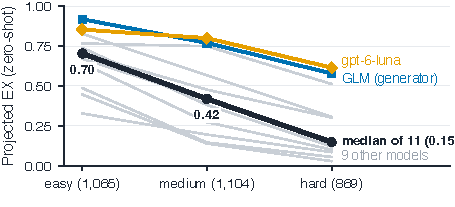
\includegraphics[width=\columnwidth]{figures/tier_accuracy.pdf}
\caption{Zero-shot projected EX on all 3,038 items by calibrated tier (item counts): all 11 models fall from easy to hard.}
\label{fig:tiers}
\end{figure}
\begin{table}[H]
\centering
\footnotesize
\begin{tabular}{@{}lrrr@{}}
\toprule
Model & Easy & Medium & Hard \\
\midrule
gpt-6-luna$^\ddagger$ & 0.85 & 0.80 & 0.61 \\
GLM-5.3-Flash$^\dagger$ & 0.92 & 0.77 & 0.58 \\
Gemma-4-26B-A4B & 0.77 & 0.75 & 0.51 \\
gpt-oss-20b & 0.83 & 0.57 & 0.30 \\
Mistral-Small-3.2-24B & 0.70 & 0.48 & 0.30 \\
Qwen3-Coder-30B-A3B & 0.74 & 0.38 & 0.12 \\
Phi-4 & 0.67 & 0.42 & 0.15 \\
Qwen3.5-9B & 0.64 & 0.27 & 0.10 \\
Llama-3.1-8B & 0.49 & 0.14 & 0.05 \\
Gemma-3-12B & 0.33 & 0.19 & 0.08 \\
Gemma-3-4B & 0.45 & 0.14 & 0.03 \\
\midrule
Median (11 models) & 0.70 & 0.42 & 0.15 \\
\bottomrule
\end{tabular}
\caption{Zero-shot projected EX on all 3,038 items by calibrated tier (1,065 easy, 1,104 medium, 869 hard), the numbers behind Figure~\ref{fig:tiers}.}
\label{tab:downstream_tiers}
\end{table}


\section{A 9B Generator Through the Same Pipeline}
\label{app:gen9b}
We ran the v3 pipeline with Qwen3.5-9B (BF16, no reasoning) as the generator of templates, questions, and references, keeping the GLM\,+\,Gemma judge panel, checks, and quotas, at 25 items per category on FinBench and SNB (seed 1). Table~\ref{tab:gen9b} compares it with the first 25 accepted items per cell of the main build's seed-1 half, generated by GLM under the same configuration. The GLM arm is cut at its 25th acceptance, so it fills every cell by construction, and its tier quotas were sized for a 125- or 75-item cell; the 9B run's quotas were sized for 25 items, which explains much of its tier-quota churn.

\begin{table}[H]
\centering
\footnotesize
\setlength{\tabcolsep}{4pt}
\resizebox{\columnwidth}{!}{%
\begin{tabular}{@{}lrr@{}}
\toprule
& Qwen3.5-9B & GLM-5.3-Flash \\
\midrule
Candidates $\rightarrow$ accepted & 2,297 $\rightarrow$ 325 & 515 $\rightarrow$ 400 \\
Acceptance rate & 14\% & 78\% \\
Cells reaching 25 items & 4 of 16 & 16 of 16 \\
Template proposals meeting the contract & 30\% & 76\% \\
\multicolumn{3}{@{}l}{\emph{First blocking reason (counts)}} \\
Tier quota full & 1,220 & 0 \\
Category contract & 321 & 2 \\
Slot bindings unavailable & 146 & 37 \\
Execution, schema, or syntax error & 98 & 0 \\
Judge panel reject & 57 & 15 \\
\multicolumn{3}{@{}l}{\emph{Accepted items}} \\
Both judges pass (of judged candidates) & 85\% & 96\% \\
Query signatures (top-10 share) & 180 (23\%) & 259 (17\%) \\
Self-BLEU-2, sampled & 0.74 & 0.79 \\
API cost per 1,000 accepted items & \$3.52 & \$0.85 \\
\bottomrule
\end{tabular}}
\caption{Qwen3.5-9B vs.\ GLM as the generator. About half of the 9B model's rejected template proposals declare slots their Cypher never uses, and its questions often break the category contract (e.g., a yes/no question whose query returns rows), so the pipeline rejects most of its candidates before the judges; what it does accept passes the same checks and panel. Given GLM's questions in the fixed-plan replay, its references return the released answer on 86\% of items, against 94\% for a second GLM run (Table~\ref{tab:validity}b).}
\label{tab:gen9b}
\end{table}

The pipeline therefore protects quality when the generator is weak, at the price of yield and cost: the 9B model is a workable reference writer but a poor template author. A tenant restricted to one 24\,GB GPU can combine the two observations by seeding templates from its query log or from schema-derived families (Appendix~\ref{app:tenant}) and letting the small model write questions and references.


\section{Wide-Schema Stress Test}
\label{app:wide}
To test schemas with more than 100 labels, we copied the five public graphs (FinBench, SNB, Recommendations, Northwind, FinCEN) four times each into one Neo4j database, namespacing every label and relationship type (e.g., \cy{FinA\_Account}, \cy{FINA\_TRANSFER\_TO}) so that every label holds real data. The merged graph has 132 labels, 148 relationship types, 372 relationship patterns, 1,116 node properties, 328,652 nodes, and 1.35M relationships; its profiled schema takes about 6,200 prompt tokens, against 800 for FinBench and 1,100 for SNB. We ran the unchanged v3 pipeline (GLM generator, GLM\,+\,Gemma-4 panel, no hand-written templates) at 10 items per category.

\begin{table}[H]
\centering
\footnotesize
\resizebox{\columnwidth}{!}{%
\begin{tabular}{@{}lrr@{}}
\toprule
& Wide (132 labels) & Main build \\
\midrule
Candidates $\rightarrow$ accepted & 135 $\rightarrow$ 80 (59\%) & 5,617 $\rightarrow$ 3,042 (54\%) \\
Cells at target & 8 of 8 & 21 of 32$^\ast$ \\
Template proposals meeting the contract & 59\% & 76\% \\
Empty-result rejections (\% of candidates) & 3.7\% & 1.3\% \\
API cost per 1,000 accepted items & \$2.13 & \$1.15 \\
Prompt tokens served from cache & 33\% & 37\% \\
Accepted queries mixing namespaces & 0 & -- \\
Accepted items flagged by the outside auditor & 29\% (23/80) & 22\% \\
\bottomrule
\end{tabular}}
\caption{The pipeline on a 132-label schema. $^\ast$Eight main-build cells were stopped at a time budget (Appendix~\ref{app:judges}). Template rejections on the wide schema are mostly properties attached to the wrong label (32 of 36), which the schema check catches. Accepted items span all five domains but unevenly (Recommendations 34, FinCEN 26, Northwind 11, FinBench 8, SNB 1), because the planner balances categories and ignores domains.}
\label{tab:wide}
\end{table}

A schema with 26 times FinBench's labels (an eight-times longer schema prompt) roughly doubles the cost per item and makes template proposals noisier; every cell still fills, and the outside auditor's flag rate rises from 22\% to 29\% on these 80 items (no human labels or downstream runs on this graph). A tenant with a schema this size would add domain quotas next to the category quotas and, beyond a few hundred labels, slice the schema per template to the labels within a few hops of its pattern.


\section{Refresh Details}
\label{app:refresh}
Table~\ref{tab:refresh} reports, for each schema migration and data-drift edit, how many stale references break and how the incremental refresh handles them. In the misestimate experiment after the \cy{TRANSFER\_TO} rename (Figure~\ref{fig:refresh}), the 11 models score a median of 17.5 points higher against stale than against refreshed references. After \cy{GUARANTEE} was dropped, regenerating the 180 affected items took 75 worker-minutes and \$0.16; rebuilding FinBench from scratch took 950 worker-minutes and \$2.06, so the refresh used about 8\% of each.
\begin{table}[H]
\centering
\footnotesize
\setlength{\tabcolsep}{3pt}
\resizebox{\columnwidth}{!}{%
\begin{tabular}{@{}lrrrrrr@{}}
\toprule
& \multicolumn{3}{c}{Stale items (\%)} & \multicolumn{3}{c}{Incremental refresh (items)} \\
\cmidrule(lr){2-4}\cmidrule(l){5-7}
Change & broken & silent & same & rewrite & re-exec. & regen. \\
\midrule
Identity control & 0.0 & 0.0 & 100.0 & 0 & 0 & 0 \\
M1 rename \cy{TRANSFER\_TO} & 29.9 & 1.4 & 68.7 & 562 & 25 & 2 \\
M2 rename \cy{isBlocked} & 22.8 & 0.0 & 77.2 & 430 & 0 & 0 \\
M3 add \cy{Merchant} label & 0.0 & 14.0 & 86.0 & 0 & 227 & 36 \\
M4 drop \cy{GUARANTEE} & 9.6 & 0.0 & 90.4 & 0 & 0 & 180 \\
D1 delete 10\% transfers & 0.0 & 15.9 & 84.1 & 0 & 295 & 4 \\
D2 add 5\% transfers & 0.0 & 12.6 & 87.4 & 0 & 235 & 2 \\
\bottomrule
\end{tabular}}
\caption{Re-executing the 1,882 stale v3 FinBench references after schema migrations (M) and data drift (D) on a copy of the graph. Broken: invalid against the new schema; Neo4j still runs them and returns empty or different rows without an error (after M1: 376 empty, 165 different, 21 unchanged of 562). Silent: valid but now returns different or no rows. Incremental refresh carries renamed items forward with a validated rewrite (after M1, 557 of 562 rewrites return the original answer), re-executes answer-only changes, and regenerates the rest.}
\label{tab:refresh}
\end{table}


\section{What the v3 Checks Would Have Caught in v2}
\label{app:v2audit}
We ran v3's literal-consistency check and tie check over the released v2 benchmark after the fact.

\paragraph{Literal mismatches.} 201 of v2's 2,080 items (9.7\%) state a value the reference does not use or use a value the question does not state. The most frequent problems (an item can have several) are malformed quoted identifiers produced by v2's id-slot phrasing (142 items), an unstated \cy{LIMIT}~$k$ (38), an unfilled template placeholder (24), a Cypher literal the question never mentions (16), a bound value missing from the Cypher (11), and numbers or hop bounds that differ (7). They concentrate in ranking (72 of 260) and negation (41 of 260). On v2's held-out test, dropping the 29 flagged items moves no model by more than 4.9 points, and model rankings barely change (Kendall $\tau$ between full and clean test: 1.00 zero-shot, 0.96 governed, 0.85 few-shot); models solve the flagged items less often (median 0.28 vs.\ 0.35 zero-shot).

\paragraph{Ties at a \cy{LIMIT} cutoff.} 65 of v2's 283 references with \cy{ORDER BY\ldots LIMIT} tie at the cutoff, and 3 bind an entity identifier as the $k$ of a top-$k$ question; dropping the 10 affected test items moves no model by more than 2.1 points. v3 rejects both before the judge (131 tie rejections in the build), and its release contains neither.


\section{Graphs and Schemas}
Table~\ref{tab:graph_statistics} gives the size of each graph, and Figures~\ref{fig:finbench_schema} and~\ref{fig:snb_schema} show the two main schemas.
\begin{table}[H]
\centering
\footnotesize
\resizebox{\columnwidth}{!}{%
\begin{tabular}{@{}lrrrrr@{}}
\toprule
Graph & Nodes & Edges & Labels & Rel.\ types & Patterns \\
\midrule
FinBench (SF0.1) & 10,006 & 57,622 & 5 & 9 & 13 \\
SNB (LDBC) & 34,735 & 70,842 & 14 & 15 & 59 \\
\midrule
Recommendations & 28,863 & 166,261 & 6 & 4 & 12 \\
Northwind & 1,035 & 3,139 & 5 & 4 & 4 \\
FinCEN & 7,524 & 40,835 & 3 & 5 & 5 \\
\bottomrule
\end{tabular}
}
\caption{Graphs, from live introspection. FinBench and SNB carry the main benchmark. The three public Neo4j example graphs have curated Text2Cypher-2024 questions and are used for the external anchor and ranking-agreement study; PIPE-Cypher onboards them with no hand-written templates. Patterns are directed start-label/type/end-label triples.}
\label{tab:graph_statistics}
\end{table}

\begin{figure}[H]
\centering
\resizebox{\columnwidth}{!}{%
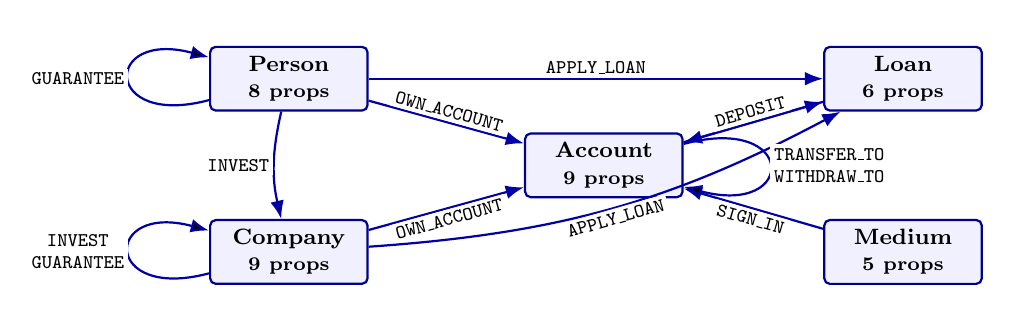
\begin{tikzpicture}[
  schemaNode/.style={draw=blue!55!black, rounded corners=2pt, fill=blue!6, thick, align=center, font=\footnotesize\bfseries, minimum width=2.0cm, minimum height=0.75cm},
  rel/.style={-Latex, thick, draw=blue!65!black},
  relLabel/.style={font=\scriptsize\ttfamily, align=center, fill=white, inner sep=1.4pt}
]
\node[schemaNode] (person) at (0,0) {Person\\{\scriptsize 8 props}};
\node[schemaNode] (company) at (0,-2.2) {Company\\{\scriptsize 9 props}};
\node[schemaNode] (account) at (4.0,-1.1) {Account\\{\scriptsize 9 props}};
\node[schemaNode] (loan) at (7.8,0) {Loan\\{\scriptsize 6 props}};
\node[schemaNode] (medium) at (7.8,-2.2) {Medium\\{\scriptsize 5 props}};

\draw[rel] (person) -- node[relLabel, above, sloped] {OWN\_ACCOUNT} (account);
\draw[rel] (company) -- node[relLabel, below, sloped] {OWN\_ACCOUNT} (account);
\draw[rel] (person) -- node[relLabel, above, sloped] {APPLY\_LOAN} (loan);
\draw[rel] (company) to[bend right=12] node[relLabel, below, sloped] {APPLY\_LOAN} (loan);
\draw[rel] (account) -- node[relLabel, above, sloped] {REPAY} (loan);
\draw[rel] (loan) -- node[relLabel, above, sloped] {DEPOSIT} (account);
\draw[rel] (medium) -- node[relLabel, below, sloped] {SIGN\_IN} (account);
\path[rel] (account) edge[loop right, min distance=15mm] node[relLabel, right] {TRANSFER\_TO\\WITHDRAW\_TO} (account);
\path[rel] (person) edge[loop left, min distance=14mm] node[relLabel, left] {GUARANTEE} (person);
\path[rel] (company) edge[loop left, min distance=14mm] node[relLabel, left] {INVEST\\GUARANTEE} (company);
\draw[rel] (person) to[bend right=13] node[relLabel, left] {INVEST} (company);
\end{tikzpicture}}
\caption{FinBench schema graph used in the reported runs. The workload is centered on financial entities, account ownership, transaction/event relationships, loans, sign-in media, guarantees, and investments.}
\label{fig:finbench_schema}
\end{figure}

\begin{figure}[H]
\centering
\resizebox{\columnwidth}{!}{%
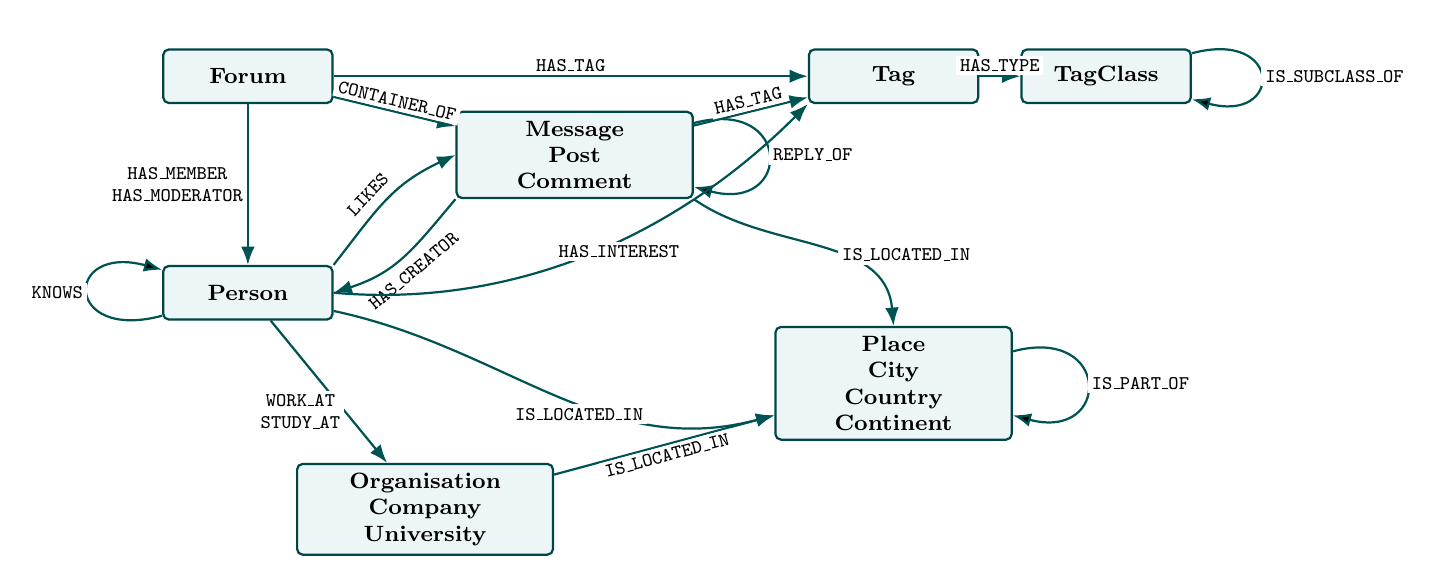
\begin{tikzpicture}[
  schemaNode/.style={draw=teal!55!black, rounded corners=2pt, fill=teal!7, thick, align=center, font=\footnotesize\bfseries, minimum width=1.85cm, minimum height=0.68cm},
  rel/.style={-Latex, thick, draw=teal!65!black},
  relLabel/.style={font=\scriptsize\ttfamily, align=center, fill=white, inner sep=1.4pt}
]
\node[schemaNode, minimum width=2.15cm] (person) at (0,0) {Person};
\node[schemaNode, minimum width=2.15cm] (forum) at (0,2.75) {Forum};
\node[schemaNode, minimum width=3.0cm] (content) at (4.15,1.75) {Message\\Post\\Comment};
\node[schemaNode, minimum width=2.15cm] (tag) at (8.2,2.75) {Tag};
\node[schemaNode, minimum width=2.15cm] (tagclass) at (10.9,2.75) {TagClass};
\node[schemaNode, minimum width=3.0cm] (place) at (8.2,-1.15) {Place\\City\\Country\\Continent};
\node[schemaNode, minimum width=3.25cm] (org) at (2.25,-2.75) {Organisation\\Company\\University};

\draw[rel] (forum) -- node[relLabel, above, sloped] {CONTAINER\_OF} (content);
\draw[rel] (forum) -- node[relLabel, left] {HAS\_MEMBER\\HAS\_MODERATOR} (person);
\draw[rel] (forum) -- node[relLabel, above, sloped] {HAS\_TAG} (tag);
\draw[rel] (content.south west) to[out=230,in=18,looseness=1.10] node[relLabel, below, sloped, pos=0.50, yshift=-2.5pt] {HAS\_CREATOR} (person.east);
\draw[rel] (person.north east) to[out=52,in=205,looseness=1.10] node[relLabel, above, sloped, pos=0.44, yshift=2.5pt] {LIKES} (content.west);
\path[rel] (content) edge[loop right, min distance=13mm] node[relLabel, right] {REPLY\_OF} (content);
\draw[rel] (content) -- node[relLabel, above, sloped] {HAS\_TAG} (tag);
\draw[rel] (person.east) to[out=-5,in=-135,looseness=0.92] node[relLabel, below, pos=0.56] {HAS\_INTEREST} (tag.south west);
\draw[rel] (tag) -- node[relLabel, above] {HAS\_TYPE} (tagclass);
\path[rel] (tagclass) edge[loop right, min distance=12mm] node[relLabel, right] {IS\_SUBCLASS\_OF} (tagclass);
\path[rel] (person) edge[loop left, min distance=13mm] node[relLabel, left] {KNOWS} (person);
\draw[rel] (person) -- node[relLabel, left, pos=0.64] {WORK\_AT\\STUDY\_AT} (org);
\draw[rel] (person) to[out=-12,in=195] node[relLabel, below, pos=0.56] {IS\_LOCATED\_IN} (place);
\draw[rel] (content.south east) to[out=-35,in=95] node[relLabel, right, pos=0.58] {IS\_LOCATED\_IN} (place.north);
\draw[rel] (org) -- node[relLabel, below, sloped] {IS\_LOCATED\_IN} (place);
\path[rel] (place) edge[loop right, min distance=13mm] node[relLabel, right] {IS\_PART\_OF} (place);
\end{tikzpicture}}
\caption{SNB schema graph used in the reported runs. Related labels are grouped into content, place, and organization families so all 14 labels and 59 directed label/type/label patterns remain readable; Table~\ref{tab:graph_statistics} gives the full inventory counts.}
\label{fig:snb_schema}
\end{figure}


\section{Example Items}
\label{app:examples}
One released item per query category follows, each chosen as the median item (by identifier) among those of its graph, category, and tier that the outside auditor passed. We then show one reference that the annotators judged wrong.
\begin{enumerate}\setlength\itemsep{2pt}
\item \textbf{Simple retrieval} (FinBench, easy). \emph{For account 276971377083286222: accountIds of accounts it transferred funds to.}
\begin{quote}\scriptsize\ttfamily\raggedright\sloppy MATCH (a\allowbreak{}:Account \{accountId\allowbreak{}: '276971377083286222'\})\allowbreak{}\allowbreak{}-[\allowbreak{}:TRANSFER\_TO]\allowbreak{}-\textgreater{}(\allowbreak{}b\allowbreak{}:Account) RETURN DISTINCT b.accountId AS accountId\end{quote}
\noindent Answer: accountId: 57983845202396614 (first of 7 rows).
\item \textbf{Complex retrieval} (SNB, medium). \emph{For cross-tag interest analysis, show the names of all tags of type ''OfficeHolder'' that persons with an interest in tag ''Max\_Mirnyi'' are also interested in.}
\begin{quote}\scriptsize\ttfamily\raggedright\sloppy MATCH (t1\allowbreak{}:Tag \{name\allowbreak{}: 'Max\_Mirnyi'\})\allowbreak{}\textless{}-\allowbreak{}[\allowbreak{}:HAS\_INTEREST]\allowbreak{}-(p\allowbreak{}:Person)\allowbreak{}-[\allowbreak{}:HAS\_INTEREST]\allowbreak{}-\textgreater{}(\allowbreak{}t2\allowbreak{}:Tag)\allowbreak{}-[\allowbreak{}:HAS\_TYPE]\allowbreak{}-\textgreater{}(\allowbreak{}\allowbreak{}:TagClass \{name\allowbreak{}: 'OfficeHolder'\})\allowbreak{} RETURN DISTINCT t2.name AS tagName\end{quote}
\noindent Answer: tagName: Gerald\_Ford (first of 25 rows).
\item \textbf{Simple aggregation} (SNB, easy). \emph{Give me the average message length in the forum titled ''Wall of David Alonso''.}
\begin{quote}\scriptsize\ttfamily\raggedright\sloppy MATCH (f\allowbreak{}:Forum \{title\allowbreak{}: 'Wall of David Alonso'\})\allowbreak{}\allowbreak{}-[\allowbreak{}:CONTAINER\_OF]\allowbreak{}-\textgreater{}(\allowbreak{}m\allowbreak{}:Message) RETURN DISTINCT avg(m.length) AS averageMessageLength\end{quote}
\noindent Answer: averageMessageLength: 107.5.
\item \textbf{Complex aggregation} (FinBench, hard). \emph{Show, for every person who repays loans, how many distinct loans they have repaid and the total repaid amount. Include person ID, loan count, and total amount, sorted by total amount descending.}
\begin{quote}\scriptsize\ttfamily\raggedright\sloppy MATCH (p\allowbreak{}:Person)\allowbreak{}-[\allowbreak{}:OWN\_ACCOUNT]\allowbreak{}-\textgreater{}(\allowbreak{}a\allowbreak{}:Account)\allowbreak{}-[r\allowbreak{}:REPAY]\allowbreak{}-\textgreater{}(\allowbreak{}l\allowbreak{}:Loan) RETURN DISTINCT p.personId AS PersonId, COUNT(DISTINCT l) AS LoanCount, SUM(r.amount) AS TotalAmount ORDER BY TotalAmount DESC\end{quote}
\noindent Answer: PersonId: 8796093023183, LoanCount: 4, TotalAmount: 256570669.11 (first of 25 rows).
\item \textbf{Boolean existence} (FinBench, medium). \emph{In the context of loan auditing: has person with id 10995116277848 applied for a loan that was deposited into an account they own? Return true or false.}
\begin{quote}\scriptsize\ttfamily\raggedright\sloppy MATCH (p\allowbreak{}:Person \{personId\allowbreak{}: '10995116277848'\})\allowbreak{}\allowbreak{}-[\allowbreak{}:APPLY\_LOAN]\allowbreak{}-\textgreater{}(\allowbreak{}l\allowbreak{}:Loan)\allowbreak{}-[\allowbreak{}:DEPOSIT]\allowbreak{}-\textgreater{}(\allowbreak{}a\allowbreak{}:Account) WHERE EXISTS \{ MATCH (p)\allowbreak{}-[\allowbreak{}:OWN\_ACCOUNT]\allowbreak{}-\textgreater{}(\allowbreak{}a) \} RETURN DISTINCT COUNT(*) \textgreater{} 0 AS result\end{quote}
\noindent Answer: result: False.
\item \textbf{Negation/difference} (SNB, hard). \emph{For our community health review, list the members of forum 'Album 6 of Lei Zhang' who have not liked any post.}
\begin{quote}\scriptsize\ttfamily\raggedright\sloppy MATCH (p\allowbreak{}:Person)\textless{}-\allowbreak{}[\allowbreak{}:HAS\_MEMBER]\allowbreak{}-(f\allowbreak{}:Forum) WHERE f.title = 'Album 6 of Lei Zhang' AND NOT EXISTS \{ MATCH (p)\allowbreak{}-[\allowbreak{}:LIKES]\allowbreak{}-\textgreater{}(\allowbreak{}\allowbreak{}:Post) \} RETURN DISTINCT p.id, p.firstName, p.lastName\end{quote}
\noindent Answer: p.id: 2199023255779, p.firstName: Jun, p.lastName: Chen.
\item \textbf{Path/temporal} (FinBench, hard). \emph{Show each company that invested in another company between 2018-01-01 and 2020-12-31 where the invested company owns no blocked account. Return the companyId of the investor and the companyId of the invested company.}
\begin{quote}\scriptsize\ttfamily\raggedright\sloppy MATCH (a\allowbreak{}:Company)\allowbreak{}-[i\allowbreak{}:INVEST]\allowbreak{}-\textgreater{}(\allowbreak{}b\allowbreak{}:Company) WHERE a \textless{}\textgreater{} b AND i.createTime \textgreater{}= datetime('2018-01-01T00\allowbreak{}:00\allowbreak{}:00') AND i.createTime \textless{}= datetime('2020-12-31T23\allowbreak{}:59\allowbreak{}:59') AND NOT EXISTS \{ MATCH (b)\allowbreak{}-[\allowbreak{}:OWN\_ACCOUNT]\allowbreak{}-\textgreater{}(\allowbreak{}acc\allowbreak{}:Account) WHERE acc.isBlocked = true \} RETURN DISTINCT a.companyId, b.companyId\end{quote}
\noindent Answer: a.companyId: 506, b.companyId: 2199023256282 (first of 25 rows).
\item \textbf{Ranking/top-$k$} (SNB, medium). \emph{Rank forums by number of members, top 5, output ID and title of each.}
\begin{quote}\scriptsize\ttfamily\raggedright\sloppy MATCH (f\allowbreak{}:Forum)\allowbreak{}-[\allowbreak{}:HAS\_MEMBER]\allowbreak{}-\textgreater{}(\allowbreak{}p\allowbreak{}:Person) WITH f, COUNT(DISTINCT p) AS memberCount ORDER BY memberCount DESC LIMIT 5 RETURN DISTINCT f.id AS forumId, f.title AS title, memberCount\end{quote}
\noindent Answer: forumId: 206158430909, title: Group for Pope\_Benedict\_XVI in Nugegoda, memberCount: 61 (first of 5 rows).
\end{enumerate}

\paragraph{A reference judged wrong.} (FinBench, path/temporal, medium.) \emph{For each pair of companies where one guaranteed the other and the guaranteed company subsequently invested in a third company, give me the guarantor companyId and the investor companyId.}
\begin{quote}\scriptsize\ttfamily\raggedright\sloppy MATCH (c1\allowbreak{}:Company)\allowbreak{}-[g\allowbreak{}:GUARANTEE]\allowbreak{}-\textgreater{}(\allowbreak{}c2\allowbreak{}:Company)\allowbreak{}-[i\allowbreak{}:INVEST]\allowbreak{}-\textgreater{}(\allowbreak{}c3\allowbreak{}:Company) WHERE i.createTime \textgreater{} g.createTime RETURN DISTINCT c1.companyId AS guarantorCompanyId, c2.companyId AS investorCompanyId\end{quote}
\noindent The question speaks of a \emph{third} company, but the query does not require the three companies to be distinct, so it can also return pairs in which the guaranteed company invests back into its guarantor. Both panel judges passed the item, the outside auditor flagged it, and the two annotators first disagreed on it and then resolved it as wrong.


\section{Prompt Contracts and Convention Sheet}
\label{app:prompts}
\label{sec:prompt_contracts}
Prompts are versioned implementation artifacts; the hashes fingerprint the prompt constants in the released code. Every v3 prompt places the fixed blocks (schema, rules, convention sheet, examples) first and the item-specific blocks last, so hosted endpoints can reuse cached prefixes; the content is not shortened.
\begin{enumerate}\setlength\itemsep{1pt}
\item \textbf{Template proposal and induction} (\texttt{007be4}, \texttt{a827ce}, rules \texttt{5b8f6e}). A question with typed slots plus parameterized Cypher that uses every slot as \cy{\$slot}; conventions C4 and C10; a requested difficulty tier; induction also lists the templates already covered and asks for structurally different ones.
\item \textbf{Question realization} (\texttt{513b36}). Rewrite in one sampled register (terse analyst, business manager, imperative, or context-first) without changing meaning; of several rewrites, the one least similar to already accepted questions is kept; every bound value verbatim; the writer rules below.
\item \textbf{Reference generation} (\texttt{f4af10}). Schema-visible constructs and observed directions only; \cy{RETURN DISTINCT} for set answers; exact equality for quoted values; required context columns; no writes; the convention sheet. The template's own Cypher, with the bound values substituted, is kept as a fallback when the generated reference is rejected, and as an agreement check otherwise.
\item \textbf{Checklist judge} (\texttt{68dd5f}, frozen before the build). Inputs: the full schema with symmetric types marked, the convention sheet, the question, the Cypher, a clause-by-clause reading the judge writes first, five result rows, and deterministic notes (unlisted patterns, variables dropped at a \cy{WITH}). The judge answers nine criteria (values, relationships, aggregation, grouping, comparisons, ranking, columns, no extra constraints, unambiguous) with yes, no, or n/a and evidence; code passes the item only if no criterion is ``no'' and ``unambiguous'' is ``yes''. Ties, truncation, emptiness, read-only safety, and syntax are left to code.
\item \textbf{Downstream Text2Cypher} (standard and governed prompts). Read-only Cypher only; schema-visible constructs and direction preservation; the governed prompt adds the generator's conventions.
\end{enumerate}

\subsection{Convention Sheet (v3.2)}
The same text is given to the question writer, the reference generator, both judges, the outside auditor, and the human annotators.
\par\smallskip
\begingroup
\fontsize{6.3}{7.3}\selectfont
\begin{verbatim}
Benchmark conventions (questions are written under these
    rules and read with them):
C1 Values. Text in quotation marks is an exact, case-
    sensitive value. Identifiers are written without
    quotation marks (for example "account
    4803651952544056659") and match the label's
    identifying property. A quoted number or boolean that
    names a value ("'73'", "'False'") means that value in
    the property's stored type. Every value the question
    states appears in the query, and the query filters on
    no literal value that the question does not state.
C2 Direction. A verb with a direction ("transferred to",
    "invested in", "owned by", "replied to", "applied
    for") fixes the relationship direction. A neutral verb
    ("connected to", "linked with", "related to",
    "associated with") means either direction; a question
    that intends one direction must use a directed verb.
    Symmetric relationship types (listed with the schema)
    are matched without a direction.
C3 Roles. A role noun ("investor", "owner", "member",
    "author") covers every label that can play that role
    in the schema unless the question names the label.
C4 Counting. "How many <entities>" counts distinct
    entities. "How many <transfers / links / relationships
    / events / times>" counts relationship or event
    instances. Sum, average, minimum, and maximum are
    taken over all matching instances, never over DISTINCT
    values, unless the question says "distinct" or
    "different".
C5 Sets. Answers are compared as sets of rows: duplicate
    rows and row order do not matter unless the question
    asks for an order ("in chronological order", "sorted
    by", "ranked"). DISTINCT in a query is never an error
    by itself.
C6 Columns. The query returns every attribute the question
    asks for, by name. Extra columns that identify or
    describe the returned entities (ids, names, types,
    status flags) are allowed. Extra filters, exclusions,
    or row limits that the question does not state are not
    allowed.
C7 Comparisons. "After", "before", "more than", "less
    than", "over", "under", "exceeds" are strict (>, <).
    "On or after", "since", "at least", "at most", "no
    more than", "up to", "until" are inclusive (>=, <=).
    "Between A and B" includes both ends. "In <year>" or
    "in <month> <year>" covers the whole period. A two-way
    split ("before and after", "above and below") may put
    the boundary value in either group.
C8 Paths. "Within N hops" means 1 to N hops; "exactly N
    hops" means N; "directly" means 1 hop. A reachability
    question states its hop bound, and the query uses
    exactly that bound.
C9 Temporal chains. "Then", "followed by", "later", or
    "subsequently" between steps require each later step's
    timestamp to be greater than the earlier step's.
C10 Self-matches. "Other", "another", "else", or
    "different" (in the sense of "not the same one")
    require the query to exclude the anchor entity, for
    example a <> b for self-transfers. Without such a
    word, the query may either allow or exclude self-
    matches; neither is an error.
C11 Ranking. "Top k by X" or "the k highest X" sorts by X
    descending and keeps k rows; "lowest", "bottom",
    "fewest" sort ascending. "Which <entity> has the most
    X" returns the maximum. The ranking is over the
    population the question names; ranking a single given
    entity against itself is degenerate and not allowed.
C12 Grouping. "For each X", "per X", or "by X" groups by X
    and returns X's identifier with each aggregate.
    Without such words an aggregate is one value over the
    whole population. Groups with zero matches are
    included only when the question says so ("including
    those with none").
C13 One reading. A question has exactly one reasonable
    reading under these conventions. It contains no
    unfilled placeholders such as {k} and no malformed
    values (such as a quoted "account with id 123"), it
    names any time window, threshold, k, or hop bound it
    relies on, and it asks only for facts the graph
    records (no "current" or historical status the schema
    does not store).
\end{verbatim}
\endgroup

\subsection{Checklist Judge Prompt}
\label{app:judgeprompt}
Both panel judges and every chat-model auditor receive the prompt below, frozen before the build. Angle brackets mark the slots filled for each item: the conventions slot holds the sheet above, and the schema slot the full profiled schema.
\par\smallskip
\begingroup
\fontsize{6.3}{7.3}\selectfont
\begin{verbatim}
[system]
You are a meticulous reviewer of
    natural-language-to-Cypher benchmark items. Return
    strict JSON only. No markdown or extra text.

[user]
Task: decide whether a benchmark item is correct. An item
    is a natural-language question and a reference Cypher
    query over the graph schema below. The item is correct
    when the query returns exactly what the question asks
    for, read under the conventions.

<conventions>

Out of scope (code checks these before you see the item;
    never answer "no" because of them): read-only safety,
    Cypher syntax, empty results, ties at an ORDER BY ...
    LIMIT cutoff, and truncation by a LIMIT without ORDER
    BY. A large LIMIT that only caps a list (the result
    has fewer rows than the LIMIT) is harmless.
    Categorical value lists constrain literals written in
    the query, not values that appear in result rows. Code
    checks that labels and properties exist and that
    simple MATCH patterns follow the schema, but it does
    not check patterns inside EXISTS / NOT EXISTS
    subqueries, untyped nodes, or whether a pattern can
    relate the entities the question means; you must check
    those.

How to review: first read the query clause by clause and
    write down what it returns: which variables each MATCH
    binds, what each WITH carries forward (a variable that
    is not carried loses its binding and matches anything
    if it is used again), which entities each mandatory
    MATCH drops, whether separate patterns are combined
    into a cross product of rows, and what one result row
    represents. Then compare that reading with the
    question.

Checklist. For each criterion, first write short evidence
    that quotes the question and the query, then answer
    "yes", "no", or "na" (na only when the criterion does
    not apply).
1. values: every entity, identifier, number, date, and
    quoted value in the question appears in the query with
    the same meaning, and the query filters on no literal
    value the question does not state (C1). A quoted
    phrase that is not itself a stored value (for example
    'account with id 123' or 'company id company') is a
    no.
2. relationships: relationship types, node labels, and
    directions express the question's meaning, and the
    pattern connects the entities the question relates
    (C2, C3). Every pattern, including patterns inside
    EXISTS / NOT EXISTS and after WITH, uses a
    relationship the schema lists between those labels in
    the listed direction (symmetric types excepted);
    variables used after a WITH were carried through it;
    independent sub-answers are not combined into a cross
    product of rows.
3. aggregation: the aggregate function and the counted
    unit match the question (C4). na if the question asks
    for no aggregate.
4. grouping: the grouping key and the per-group output
    match the question (C12). A question that asks for one
    overall value gets one value, not one per entity; a
    per-entity question is not collapsed into one value.
    na if there is neither grouping nor an overall
    aggregate.
5. comparisons: comparison operators, boundaries, time
    windows, and hop ranges match the question (C7, C8,
    C9). na if there are none.
6. ranking: the sort key, sort direction, and k match the
    question (C11). A ranking whose population is
    restricted to one given entity (for example "among
    accounts with id 123, which have the most ...") or
    whose sort key is the same for every row is a no. na
    if the question asks for no ranking or ordering.
7. columns: the query returns every attribute the question
    asks for (C6).
8. no_extra_constraints: the query adds no filter,
    exclusion, hop bound, or row limit that the question
    does not state and the conventions do not require (C6,
    C8, C10), and no mandatory MATCH drops entities the
    question asks for (for example, keeping only a
    person's comments that reply to comments when the
    question asks for all of their comments).
9. unambiguous: the question has one reasonable reading
    under the conventions, contains no unfilled
    placeholder, asks only for facts the graph stores (no
    "current" job, change history, or population the
    schema lacks), and its answer is meaningful to an
    analyst (C11, C13).

Output: one JSON object with exactly these keys:
{"query_reading": "walk through the query clause by clause
    (each MATCH pattern as start label, type, end label;
    each WITH and what it carries; each WHERE; the
    RETURN), then say what one result row represents and
    which rows are kept or dropped", "values":
    {"evidence": "...", "answer": "yes|no|na"},
    "relationships": {"evidence": "...", "answer": "..."},
    "aggregation": {...}, "grouping": {...},
    "comparisons": {...}, "ranking": {...}, "columns":
    {...}, "no_extra_constraints": {...}, "unambiguous":
    {...}, "clarified_question": "if unambiguous is no,
    one rewrite of the question that has a single reading
    and matches the query; otherwise an empty string",
    "difficulty": "easy|medium|hard"}

Graph schema:
<schema>

Item to review
Question:
<question>

Reference Cypher:
<cypher>

Result: <row_summary>
<rows>

Query features (from the parser): <features>
Validator notes: <notes>

Return the JSON object now.
\end{verbatim}
\endgroup


\end{document}
